\chapter{METHODOLOGY}
 \label{Chapter 4}
 \lhead{Chapter 4. \emph{Methodology}}

In this chapter, we will discuss the implementation of our proposed system. At first, we will describe the hardware setup used for collecting user data. Different aspects of the dataset were mentioned in the next subsection. Later, we discussed how we extracted, processed, calibrated, and denoised the raw data and made them usable for our model. Finally, a brief overview of our proposed model and approach is given.

\section{Hardware Setup}
The main hardware we used for this system is a pair of ESP32 MCU manufactured by espressif. The specific model of the used hardware module is ESP32-WROOM-32E. This is an ESP32-D0WD-based module with Wi-Fi 802.11 b/g/n and Bluetooth LE 4.2 connectivity and a dual-core processor. Traditional research on Wi-Fi-based human activity recognition uses Intel 5300 or Atheros 9390 Network Interface Card (NIC) of a laptop computer \cite{10.1145/3310194, 9264288, 9060143, 8873550, 10.1145/2789168.2790093} which is not a realistic choice for practical use because each node is a computer. The device we used is small, low-cost, programmable, and deployment-friendly and the whole system needs only one computer to process the data. 

For our experiment, we need to send CSI data from one ESP32 device to another. But ESP32 does not transmit CSI data with the initially provided firmware. So, a customized firmware by Espressif Systems \cite{esp-csi} is flashed to the devices to enable the transmission of CSI data. CSI data can be received using three ways:
\begin{enumerate}

\item \textbf{Get router CSI data:} In this process, a router is used to send CSI data to the ESP32. Firstly, the ESP32 device sends a Ping request to the router with an empty ICMP packet. The router acknowledges the request by sending a Ping Replay back to the requesting device. The CSI information is transmitted with the Ping Replay. One disadvantage of this process is that we need an extra router device and set it up separately to send CSI data.

\begin{figure}[H]
\centering
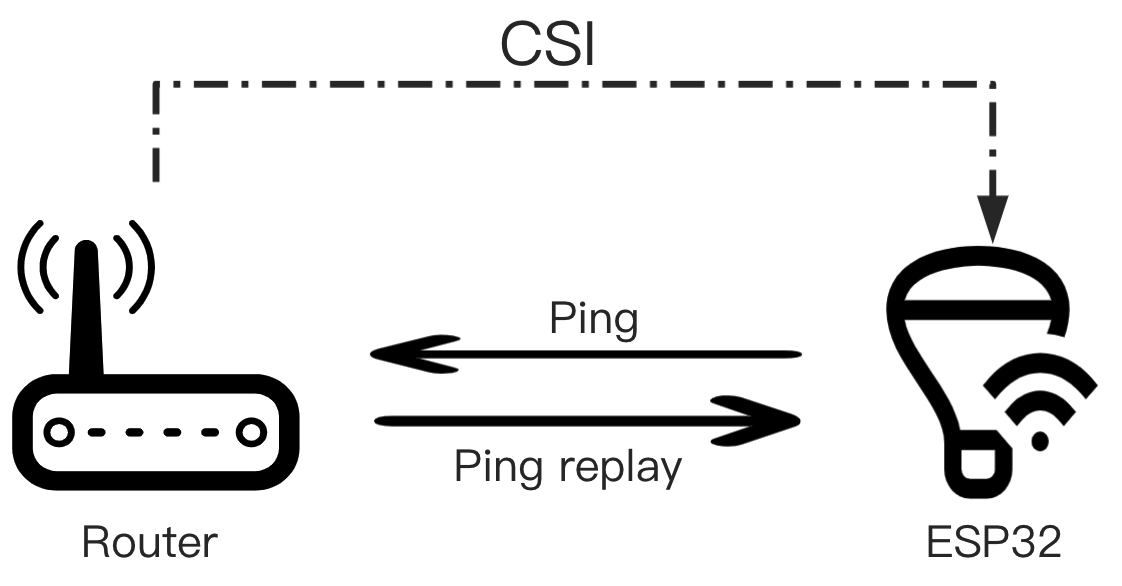
\includegraphics[width=1.0\textwidth]{./figure/chap 4/get_router_csi.png}
\caption{Get CSI data of the router}
\label{Fig 4.1}
\end{figure}

\item \textbf{Get device CSI data using router:} To implement this method, we need two ESP32 devices. ESP32 A and B both send Ping packets to the router, and ESP32 A receives the CSI information carried in the Ping Replay returned by ESP32 B. In this method, the CSI data is passed from ESP32 A to ESP32 B using an intermediate router. This intermediate connection may reduce the packet receiving rate of the system.

\begin{figure}[H]
\centering
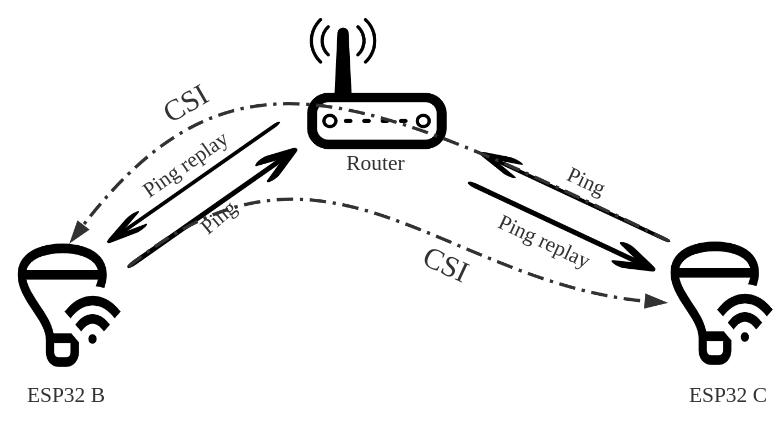
\includegraphics[width=1.0\textwidth]{./figure/chap 4/get_device_csi.png}
\caption{Get CSI data between devices using a router}
\label{Fig 4.2}
\end{figure}

\item \textbf{Get device CSI data using broadcasting:} In this method, one ESP32 device acts as a transmitting device and all other devices are receiving device. The transmitting ESP32 A sends CSI data using broadcasting. This method has the highest detection accuracy and reliability and does not require any router device. 

\begin{figure}[H]
\centering
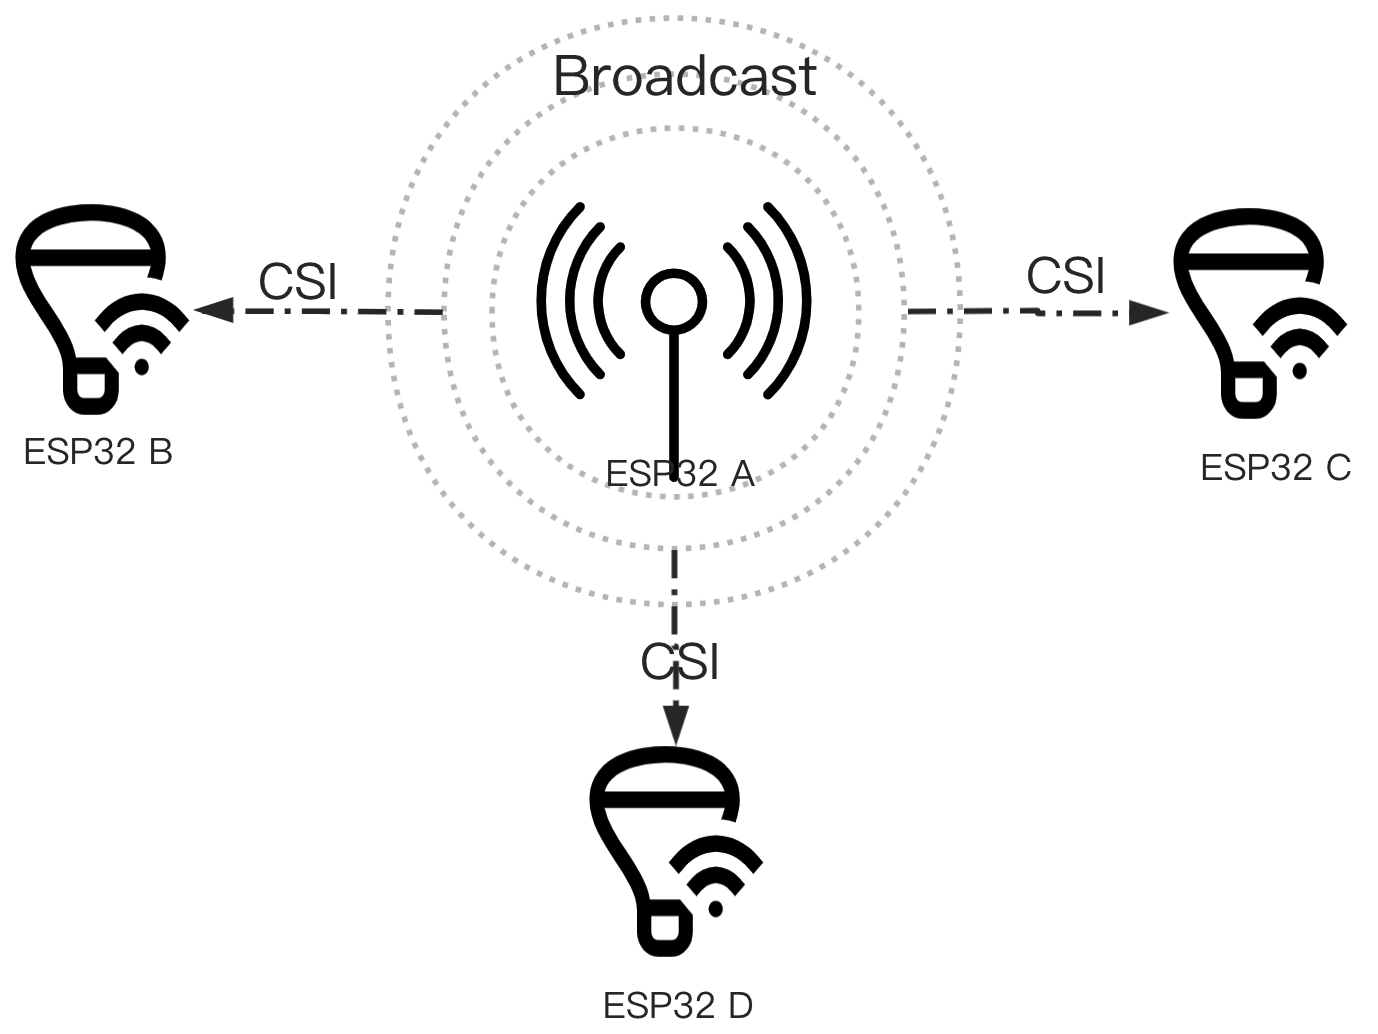
\includegraphics[width=1.0\textwidth]{./figure/chap 4/get_broadcast_csi.png}
\caption{Get CSI data using a broadcasting ESP32}
\label{Fig 4.3}
\end{figure}

\end{enumerate}

As we focus on reliability and accuracy, we choose the third method by making one ESP32 device a broadcaster and the other a receiver. We added an extra layer of security by specifying the Media Access Control (MAC) address of the receiving ESP32. As a result, if the receiving device is in the coverage area of the transmitting device, it gets CSI data automatically from the transmitting device. No overhead is required here.

        \begin{figure}[H]
        \centering
        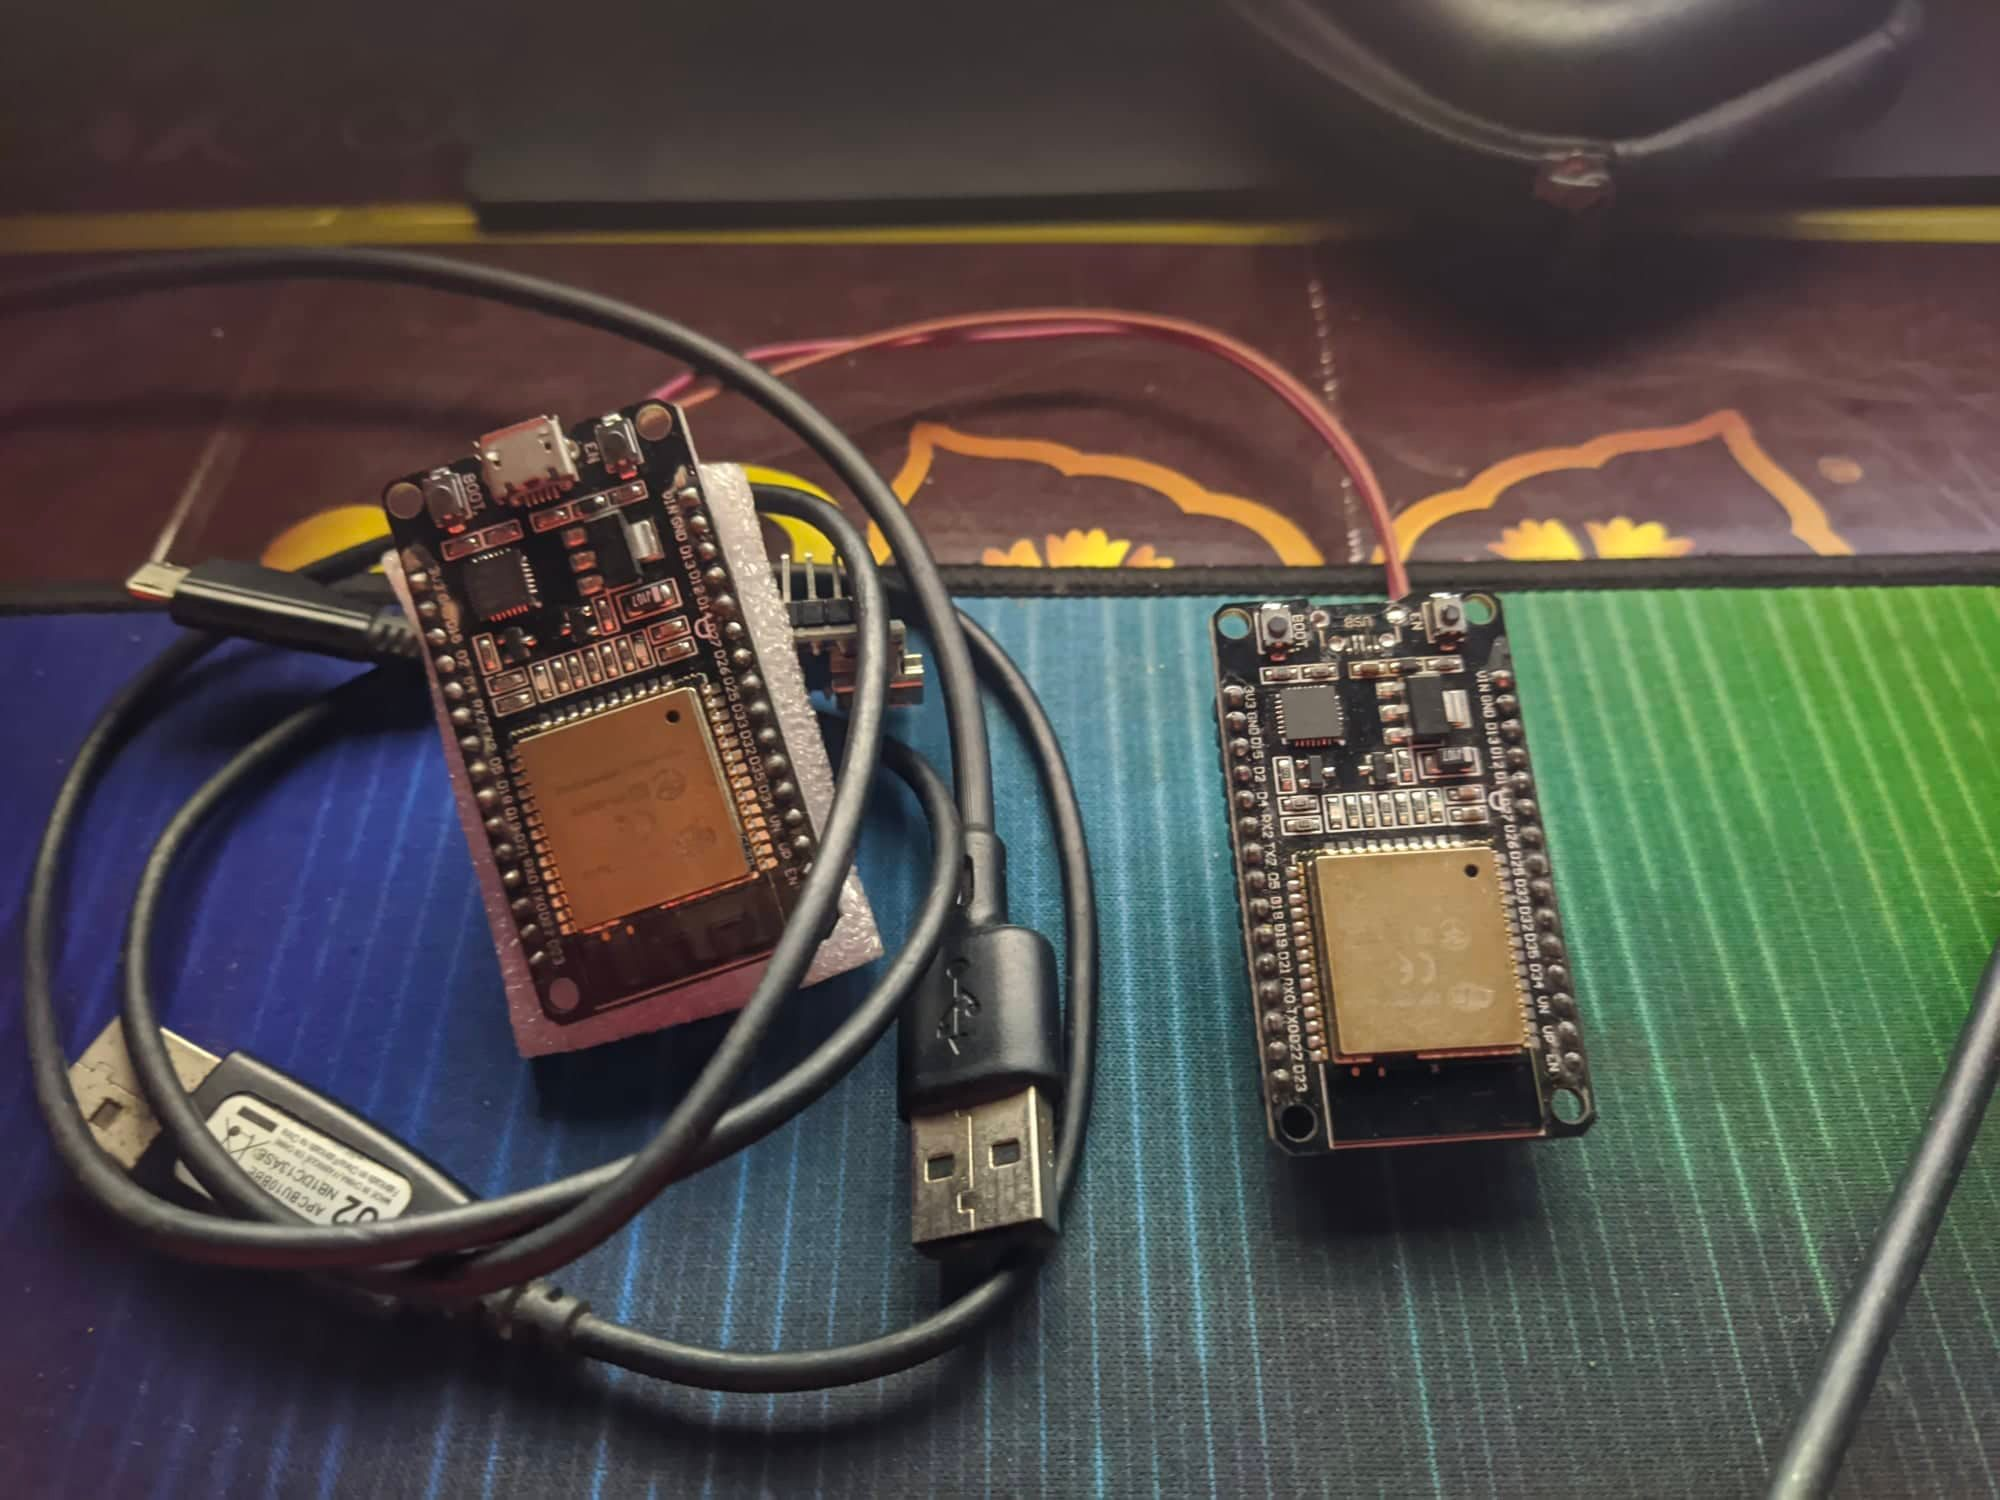
\includegraphics[width=1\textwidth, trim={0 0 0 6cm}, clip]{./figure/chap 4/myesp.jpg}
        \caption{ESP32 devices used in the project}
        \label{Fig 4.4}
        \end{figure}


Each ESP32-WROOM-32E module has one built-in PCB antenna that can transmit or receive data. It is also possible to connect any external antenna with 50 $\Omega$ resistance. In this experiment, we restricted our study to the built-in PCB antenna. We used two ESP32 modules placed approximately 3.5 meters apart. One of them is used as a transmitting device connected to any power source, and the other as a receiving device connected to a computer to process the data and predict the activity. The space between the devices is kept empty for ensuring the Line-of-Sight (LoS). The subjects are instructed to do the activities in the 3.5 meters $\times$ 3.5 meter area between the transmitting and receiving devices. Because of the movement of the subject, the transmitting packets face multipath fading, scattering, reflection, and power loss. The Channel State Information (CSI) of each packet can be analyzed to find patterns between the transmitting packets using machine learning algorithms and thus recognize the activity performed by the subject.

        \begin{figure}[H]
        \centering
        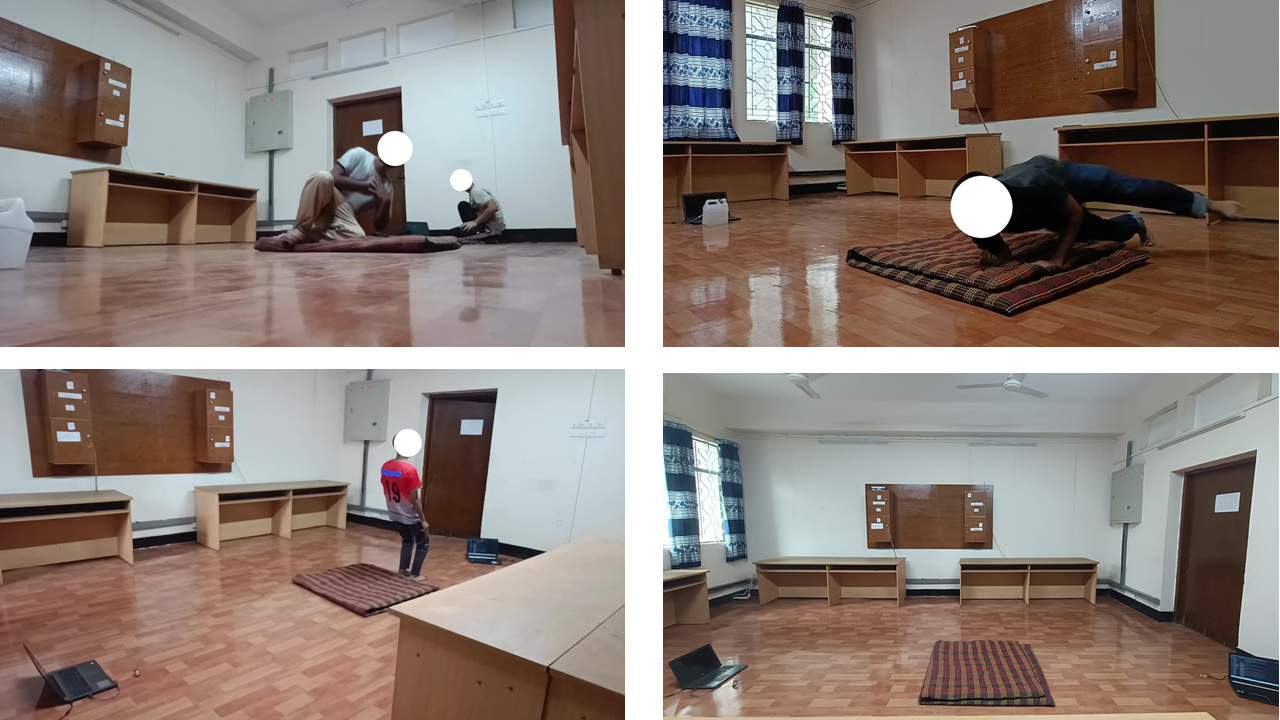
\includegraphics[width=1\textwidth]{./figure/chap 4/dataCollection.png}
        \caption{Data Collection Setup and Data Collection Example}
        \label{Fig 4.5}
        \end{figure}


ESP32-WROOM-32E supports Wi-Fi 802.11 b/g/n standards. For our experiment, we used 802.11n standard that provides support for OFDM, MIMO, frame aggregation, and higher data rate. But ESP32 does not support 5 GHz band and only works with 2.4 GHz band. The ESP32 devices we used in this experiment are configured to send data according to the following specifications:

\begin{table}[H]
\caption{Customized signal specification of ESP32}
\vspace{2mm}
\centering
\begin{tabular}{|l|l|} 
\hline
\multicolumn{1}{|c|}{\textbf{Specification}} & \multicolumn{1}{c|}{\textbf{Value}}                                                             \\ 
\hline
Standard               & IEEE 802.11n   \\
Band                   & 2.4 GHz        \\
Channel                & 20 MHz         \\
MCS index              & 0              \\
Guard interval         & 400 ns         \\
Data rate              & 7.2 Mbit/s     \\
Modulation             & BPSK           \\
Sampling rate          & 100 Hz         \\
Coding rate            & 1/2            \\
Spatial streams        & 1              \\
\hline

\end{tabular}
\label{Table 4.1}
\end{table}


\section{Dataset Description}
The accuracy and effectiveness of any data-driven study depend much on a well-prepared dataset. But there are only a few open datasets available for activity recognition using ESP32 CSI data. But these datasets do not have enough data or provide the activities we need for this system. Hence, we prepared our dataset using the hardware setup stated in the previous section. Wi-Fi CSI data is very sensitive to the outside environment which makes it very hard to collect data in the wild. Even rooms with different arrangements may affect the CSI data differently which may create a problem if a huge amount of data is not taken. For this project, we selected a neat and spacious room with minimum furniture and other things to collect the data. Two ESP32 devices are placed 3.5 meters apart and the activities are performed by different subjects in the area between the two devices. There are a total of 5 activities performed by 13 individual subjects. Each activity segment is recorded for a fixed time window of 4 seconds. This time window is chosen empirically by the type and complexity of the activities. A total of 966 samples of such segments are recorded on different calendar days.

\subsection{Challenges}
ESP32 sends Ping packets with CSI data at a rate of 100 Hz. But due to interference, unavailability of Line of Sight, and other issues, some packets are lost. As a result, though ideally each data segment of 4 seconds should have a total of $ 4 \times 100 = 400$ packets, most of the segments had packets between 300 to 340 due to packet loss.

\begin{figure}[H]
\centering
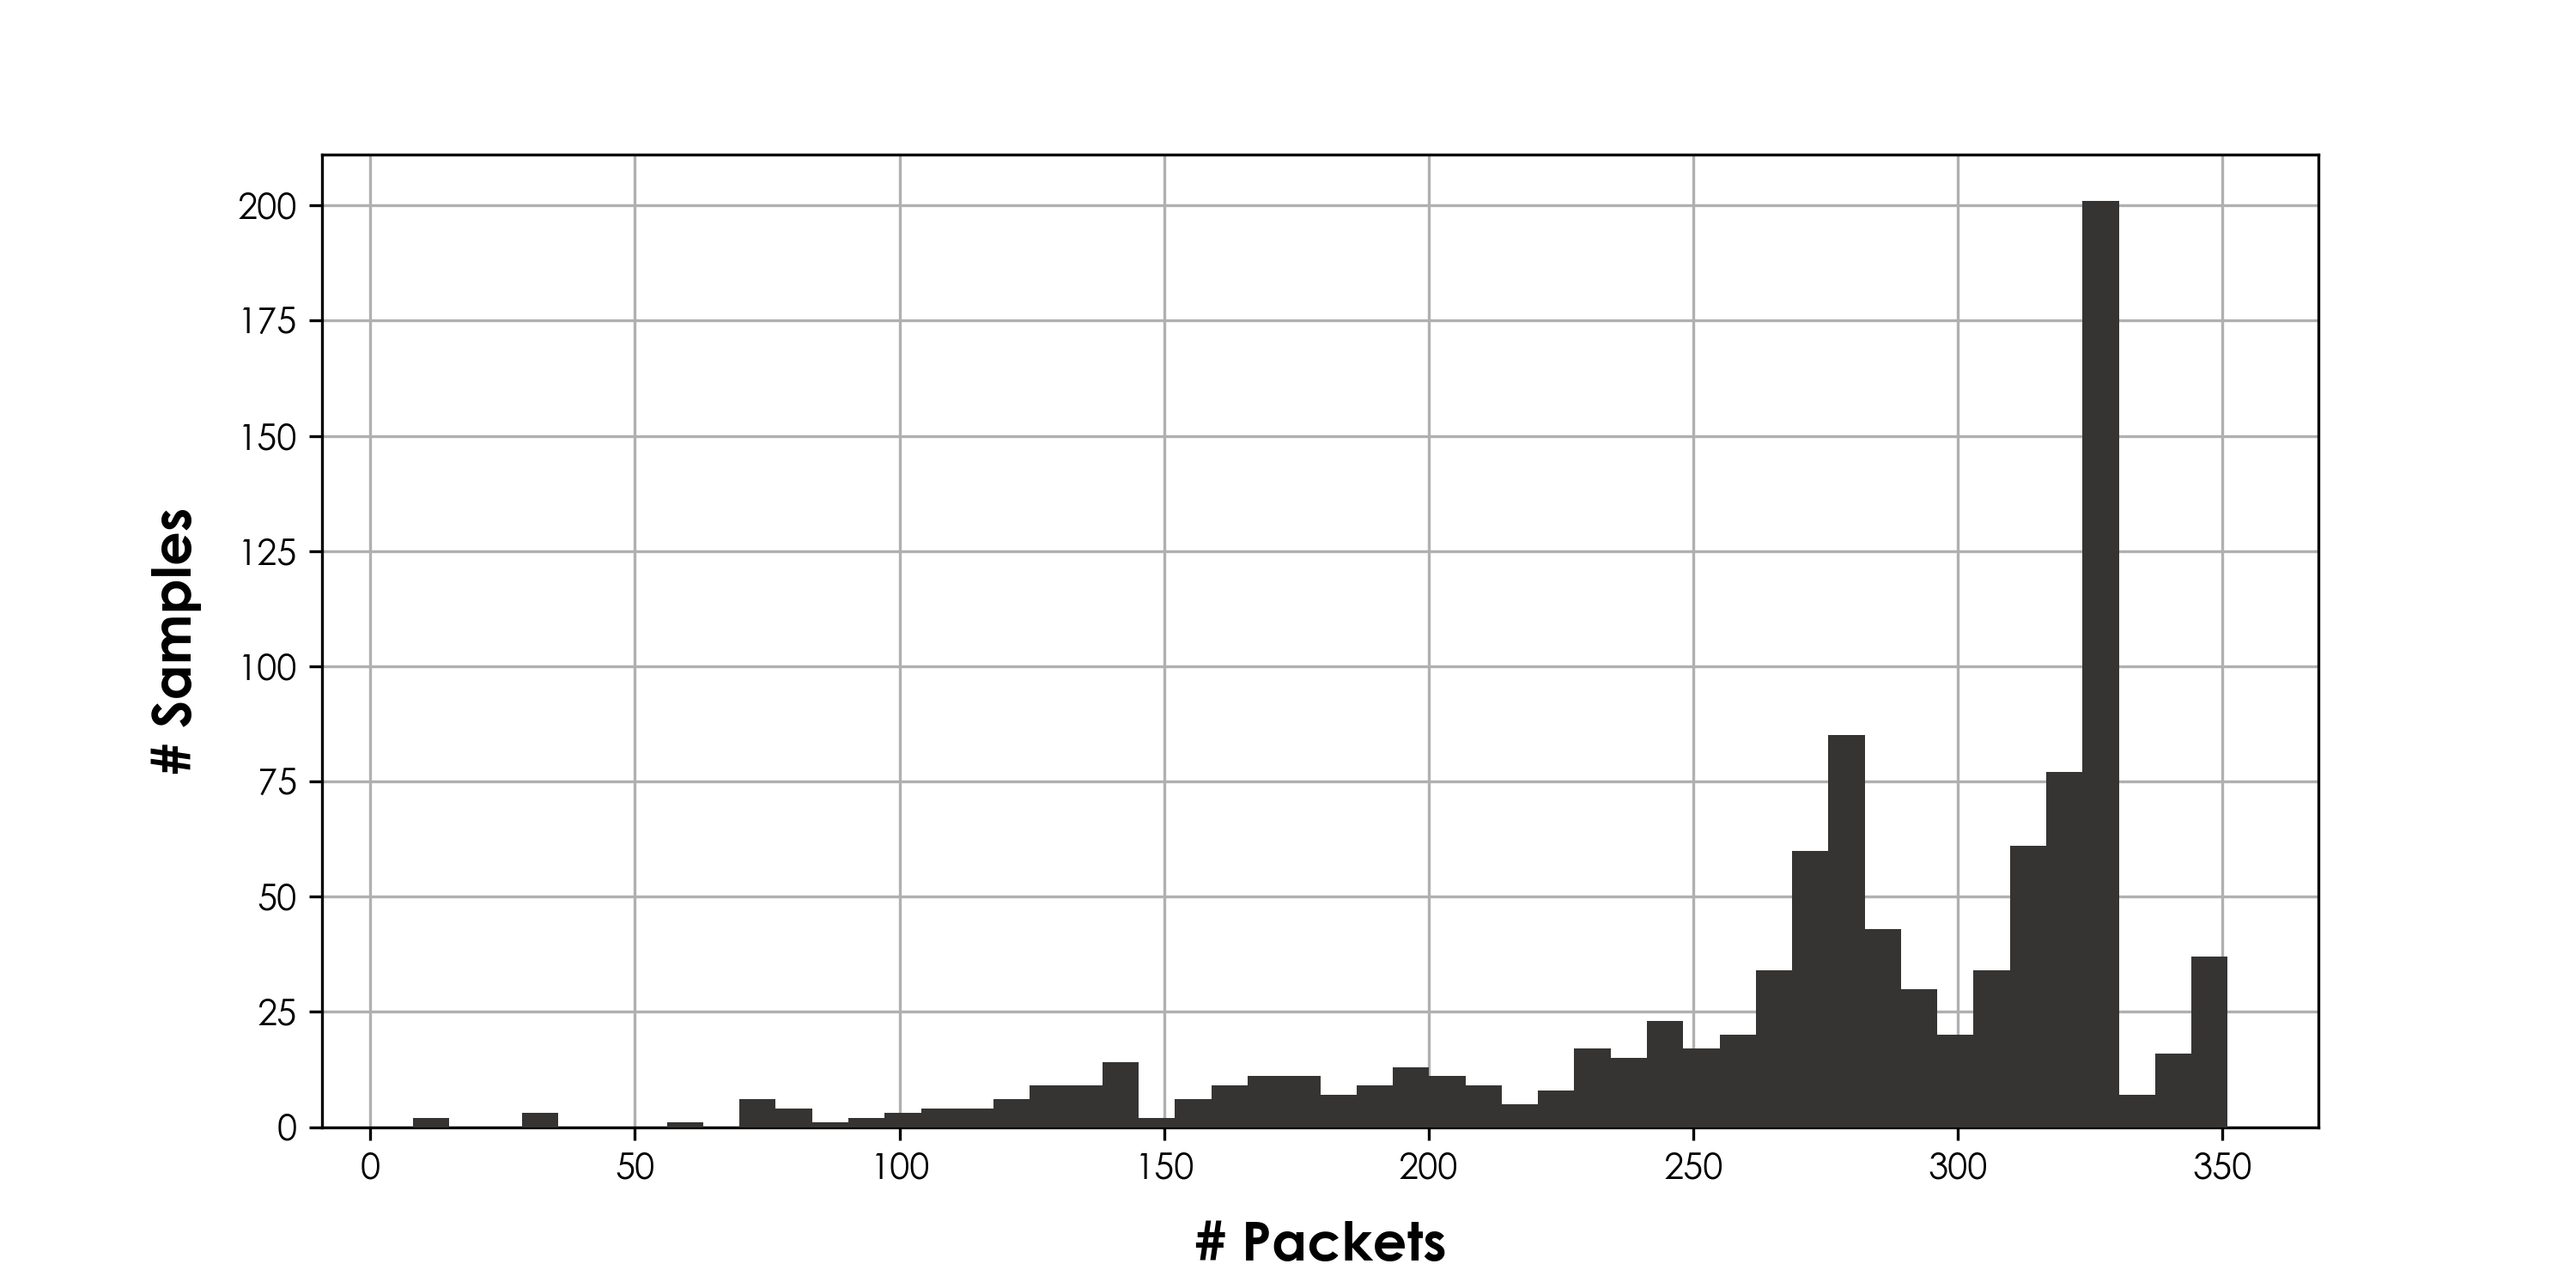
\includegraphics[width=1.0\textwidth]{./figure/chap 4/all_data_sizes.png}
\caption{Distribution of number of packets in all the collected samples}
\label{Fig 4.6}
\end{figure}

The problem here is, some of the data samples had extremely lower number of packets that were not usable in the system. So, we discarded 68 data samples with less than 150 packets. Finally, the remaining 898 data samples were used in the next steps. 

\begin{figure}[H]
\centering
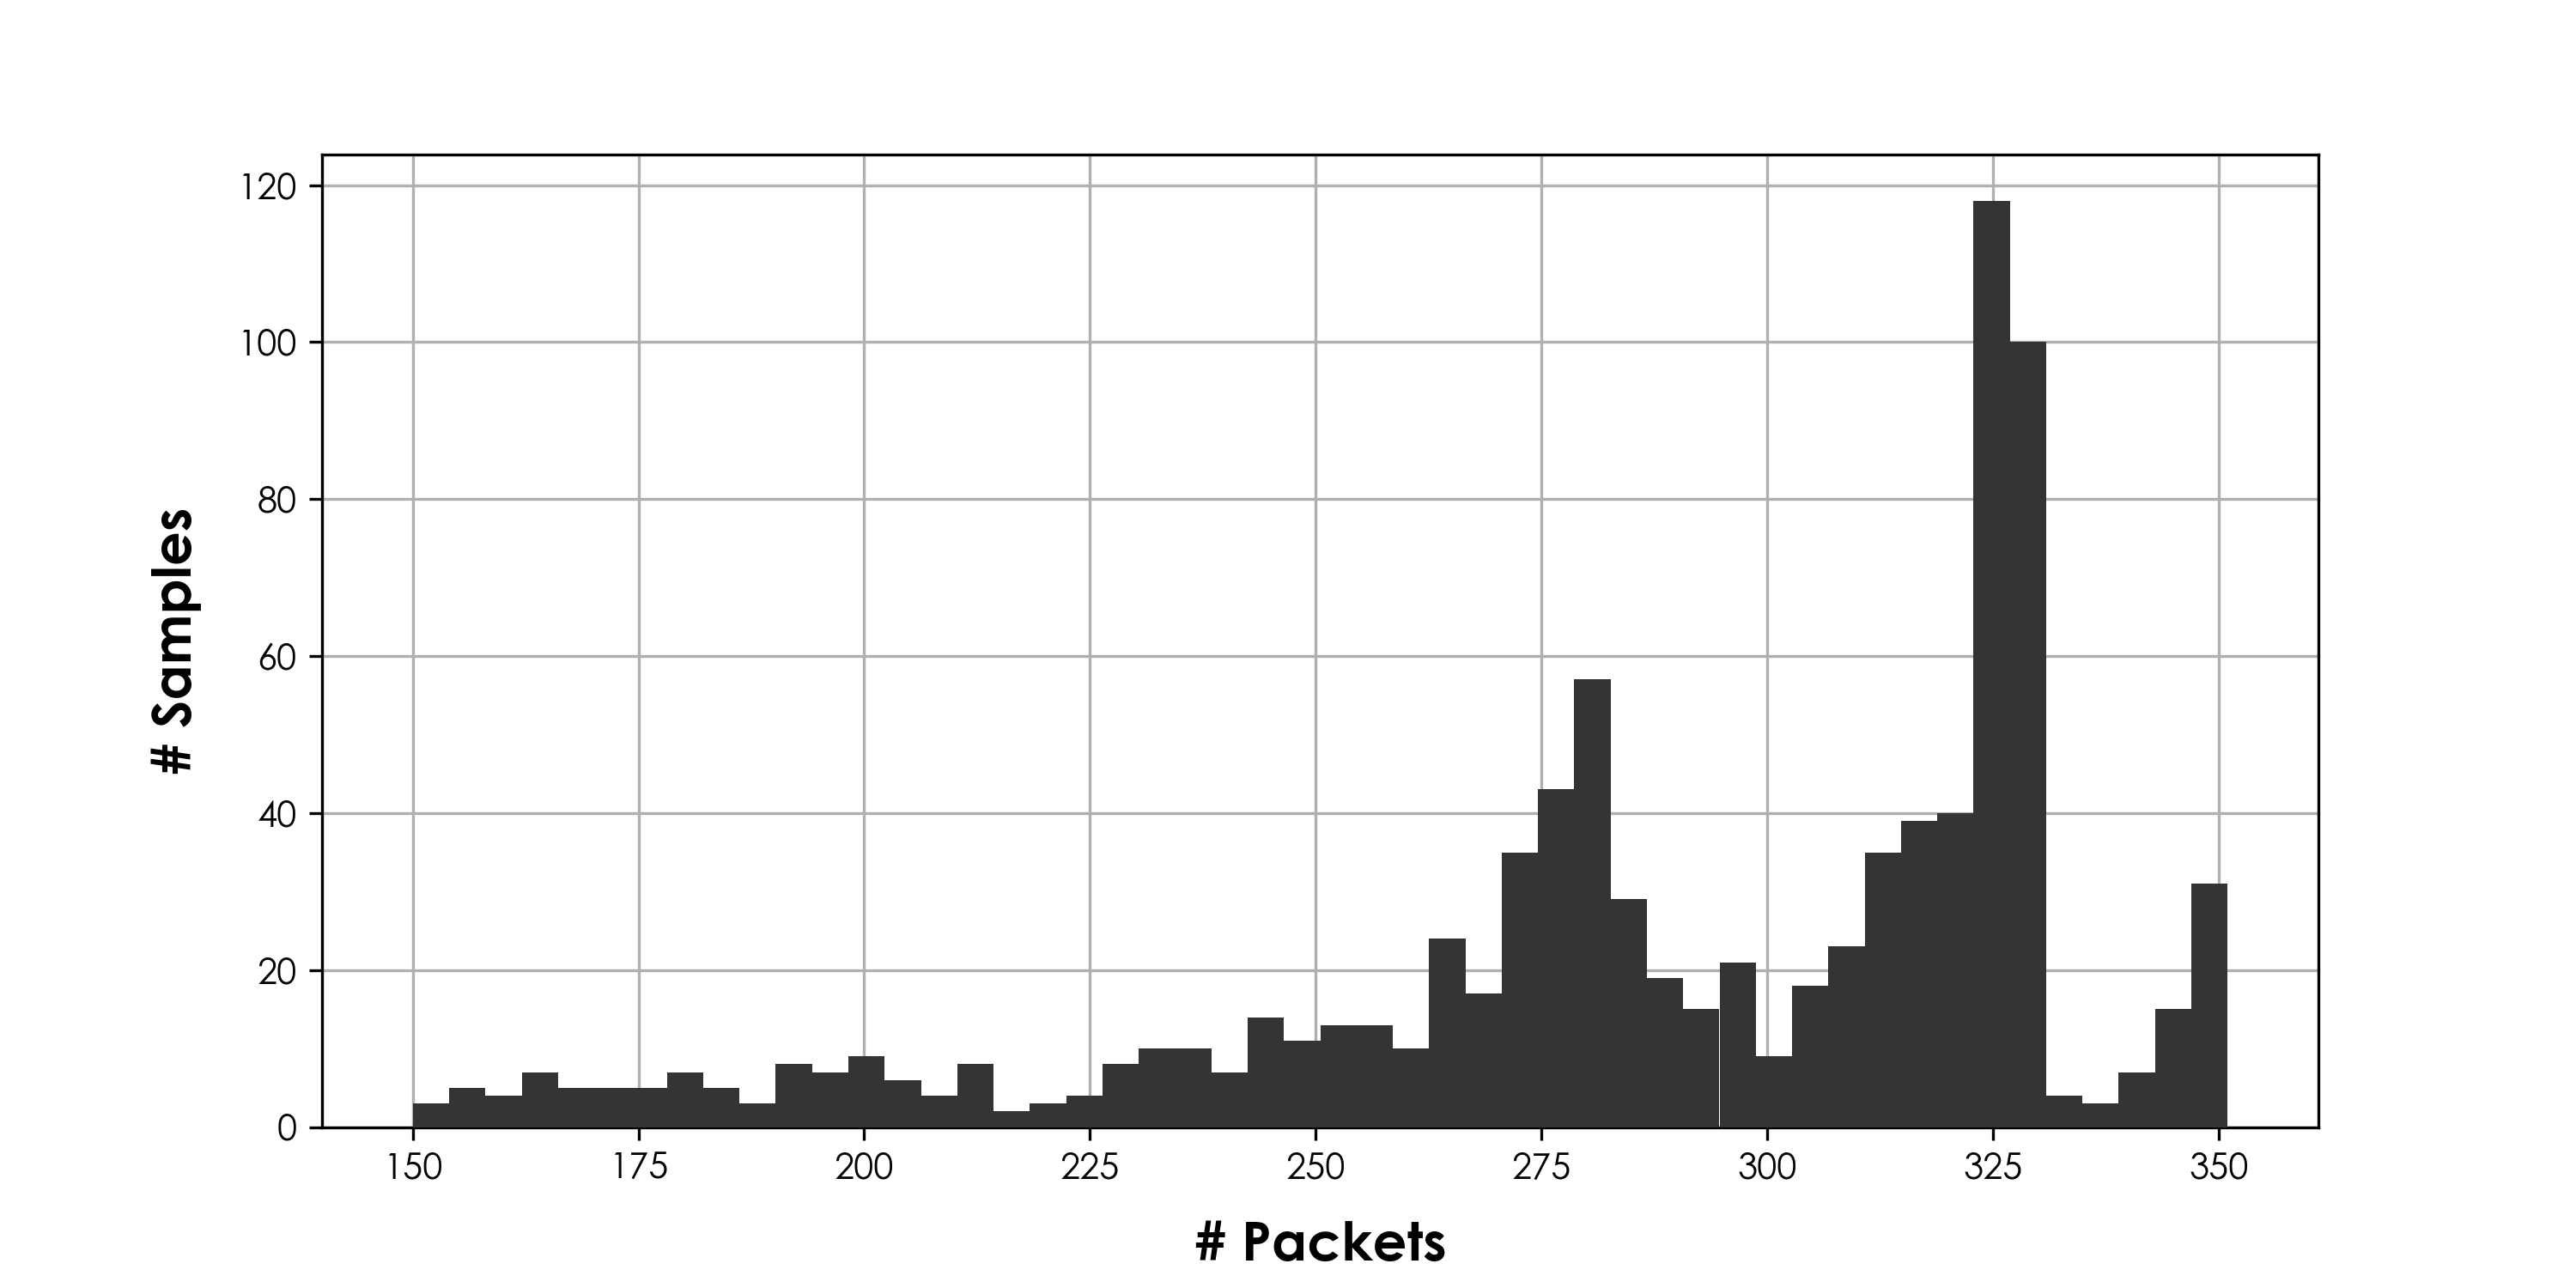
\includegraphics[width=1.0\textwidth]{./figure/chap 4/selected_data_sizes.png}
\caption{Distribution of number of packets in the selected samples}
\label{Fig 4.7}
\end{figure}

\subsection{Activities}
There are a total of 5 activities in this dataset: \emph{Fall}, \emph{Stand}, \emph{Walk}, \emph{Empty Room} and \emph{Presence}. \emph{Fall}, \emph{stand} and \emph{walk} activities are performed by one subject for each sample. For \emph{empty room} activity, no subject was present in the room. For \emph{presence}, a few subjects were present in the room doing various daily activities including gossiping, taking rest, writing, etc. Every activity excluding the \emph{empty room} was done in a different direction and fashion to preserve generality. The number of samples for each of the activity are not the same and is shown below in \ref{Table 4.2}.

\begin{table}[H]
\caption{Number of samples by activity}
\vspace{2mm}
\centering
\begin{tabular}{|l|c|} 
\hline
\multicolumn{1}{|c|}{\textbf{Activity}} & \multicolumn{1}{c|}{\textbf{Number of samples}}                                                      \\ 
\hline
Fall                   & 224            \\
Stand                  & 100            \\
Walk                   & 133            \\
Empty room             & 299            \\
Presence               & 142            \\
\hline
\end{tabular}
\label{Table 4.2}
\end{table}

\begin{figure}[H]
\centering
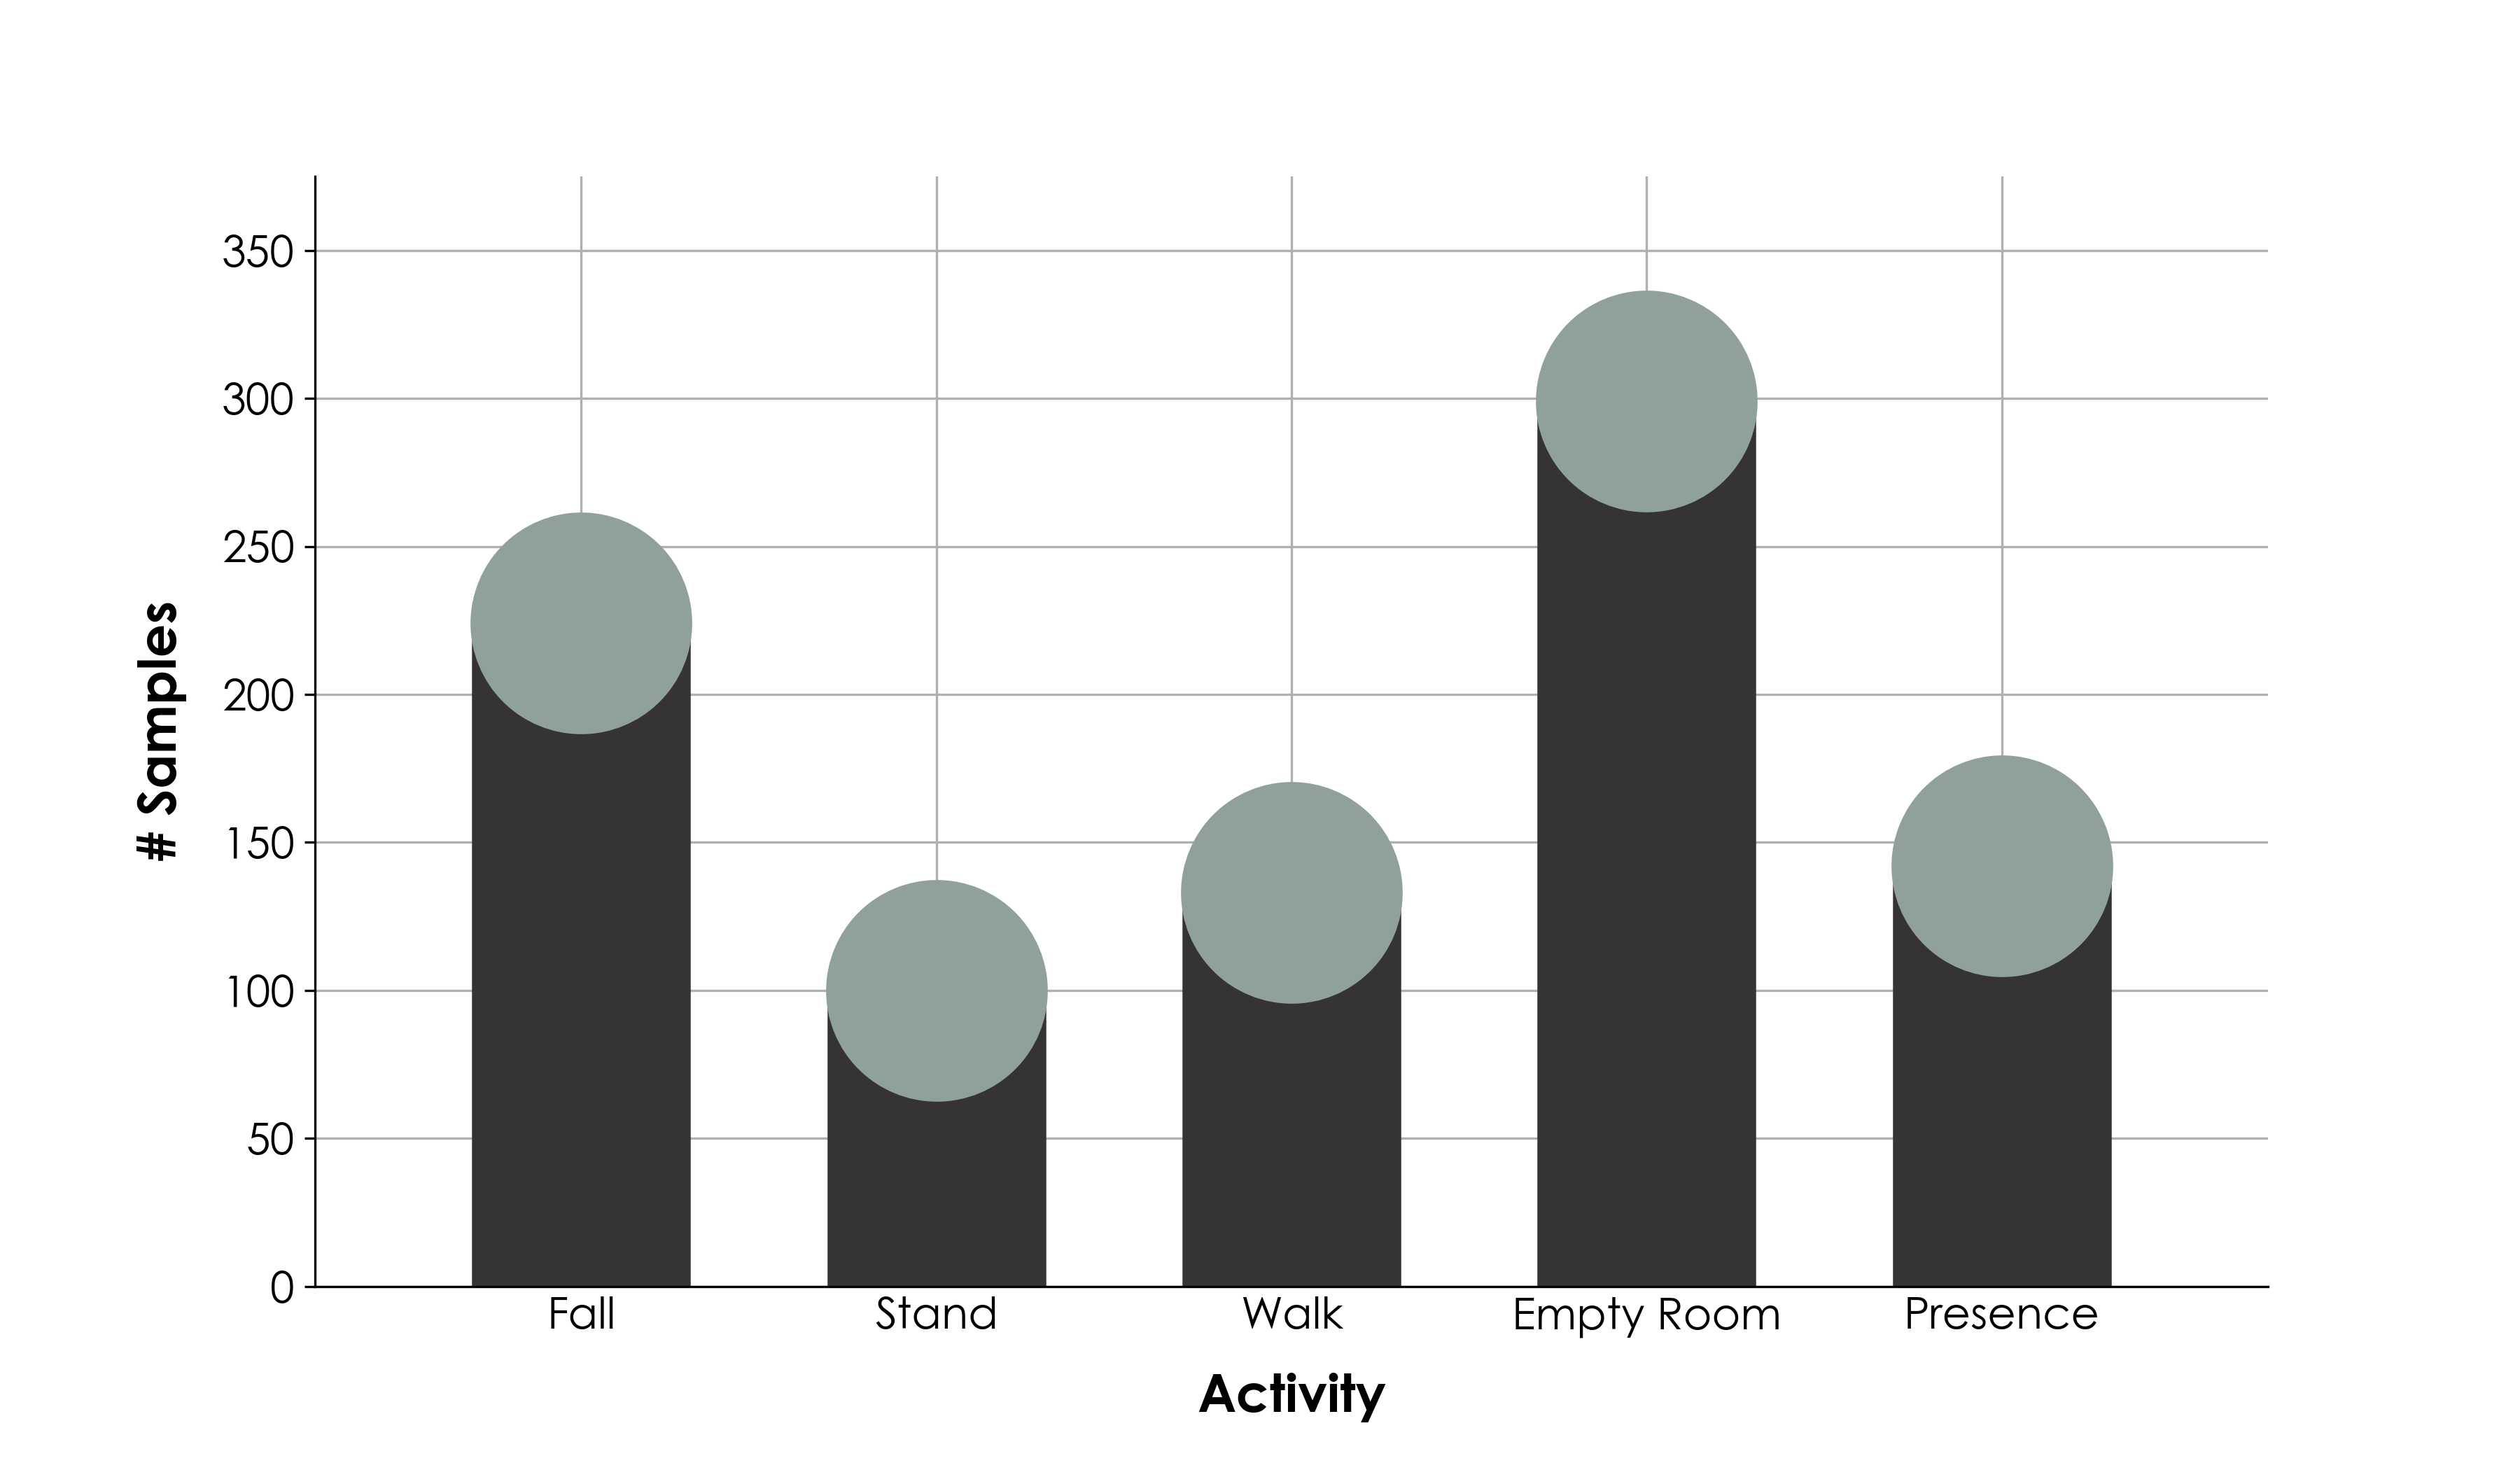
\includegraphics[width=1.0\textwidth]{./figure/chap 4/labelwise_data_counts.png}
\caption{Number of samples by activity}
\label{Fig 4.8}
\end{figure}

Packet size distribution is also different for different types of activities. As subcarriers experience a different level of scattering, reflection, or delay for different types and speeds of movement, packet loss will also be different. For example, \emph{stand} activity involves a very small amount of movement, but there should be a much higher level of movement in \emph{fall} activity. This difference in movement causes a difference in packet loss and segment size as illustrated in \ref{Fig 4.9}.

\begin{figure}[H]
\centering
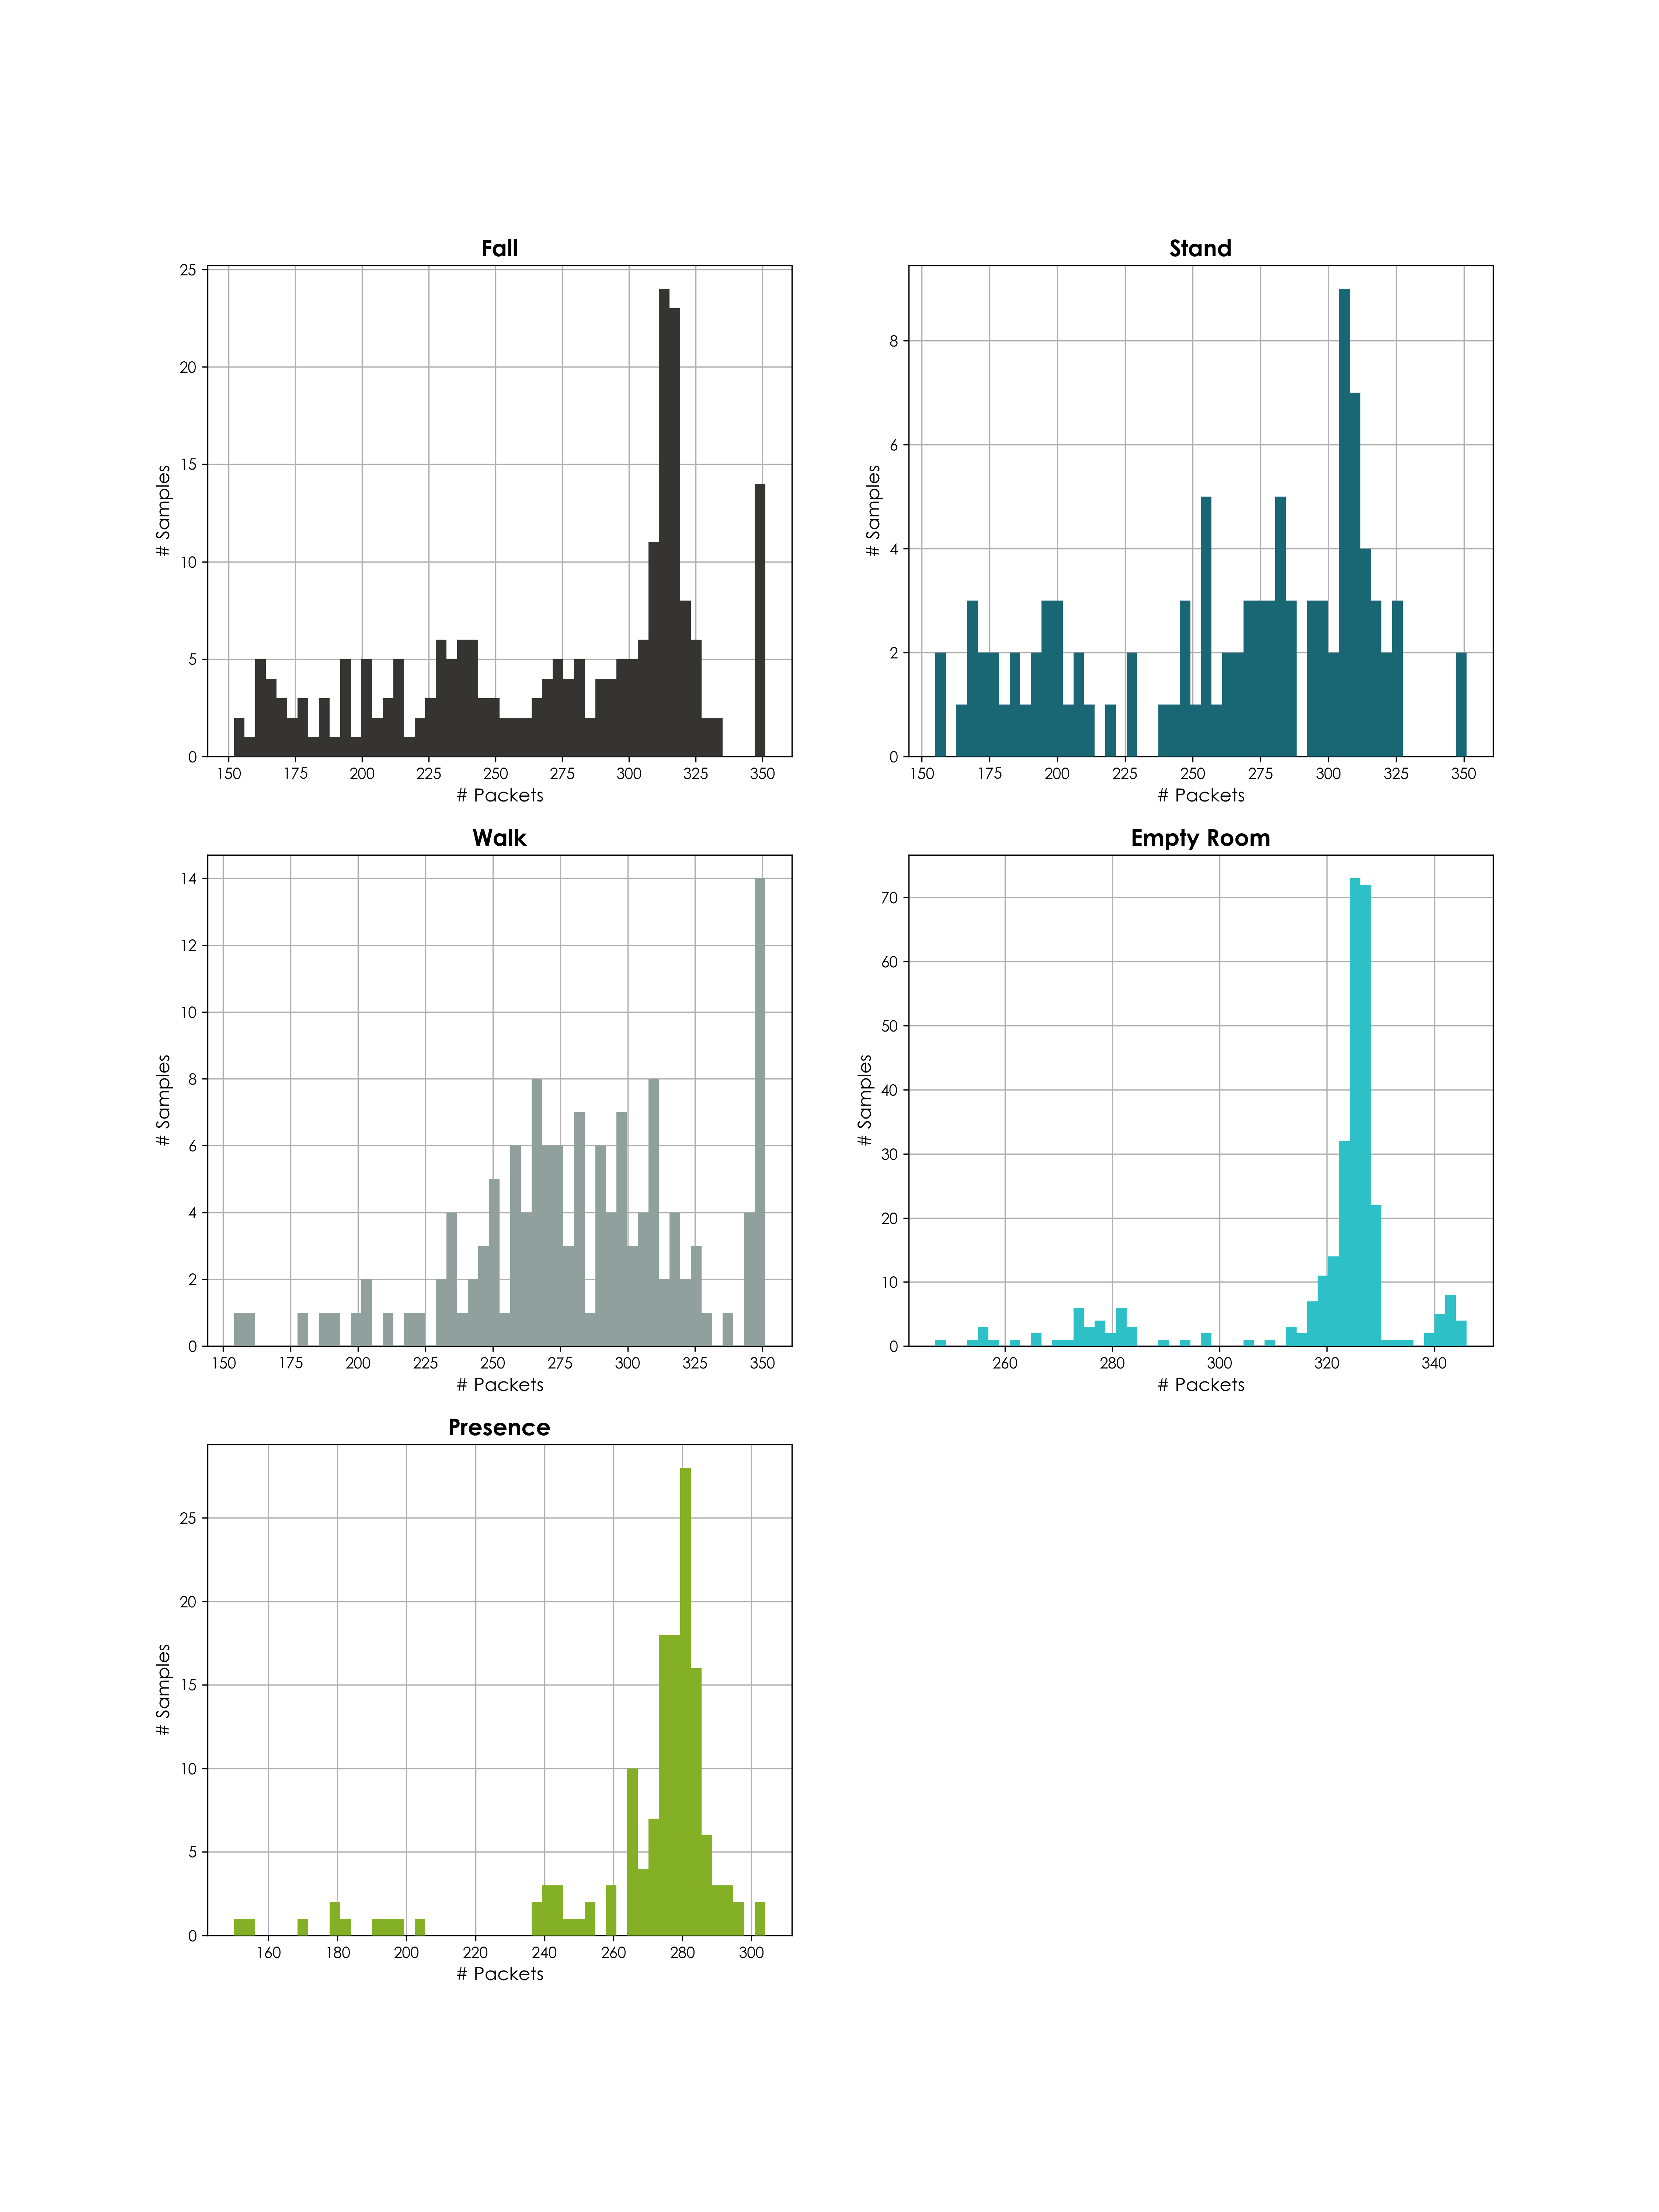
\includegraphics[width=1.0\textwidth, trim={0 6cm 0 4cm},clip]{./figure/chap 4/activity_data_sizes.png}
\caption{Packet counts of segments for different activities}
\label{Fig 4.9}
\end{figure}

\subsection{Subjects}
The number of subjects is an important aspect of any dataset. A higher number of subjects increase the generalized performance of any system. 13 subjects voluntarily performed different activities for this dataset. Most of the subjects have performed three different activities and some of them performed two or four activities out of five. In total, the subjects performed 20 to 45 segments of different activities.

\begin{figure}[H]
\centering
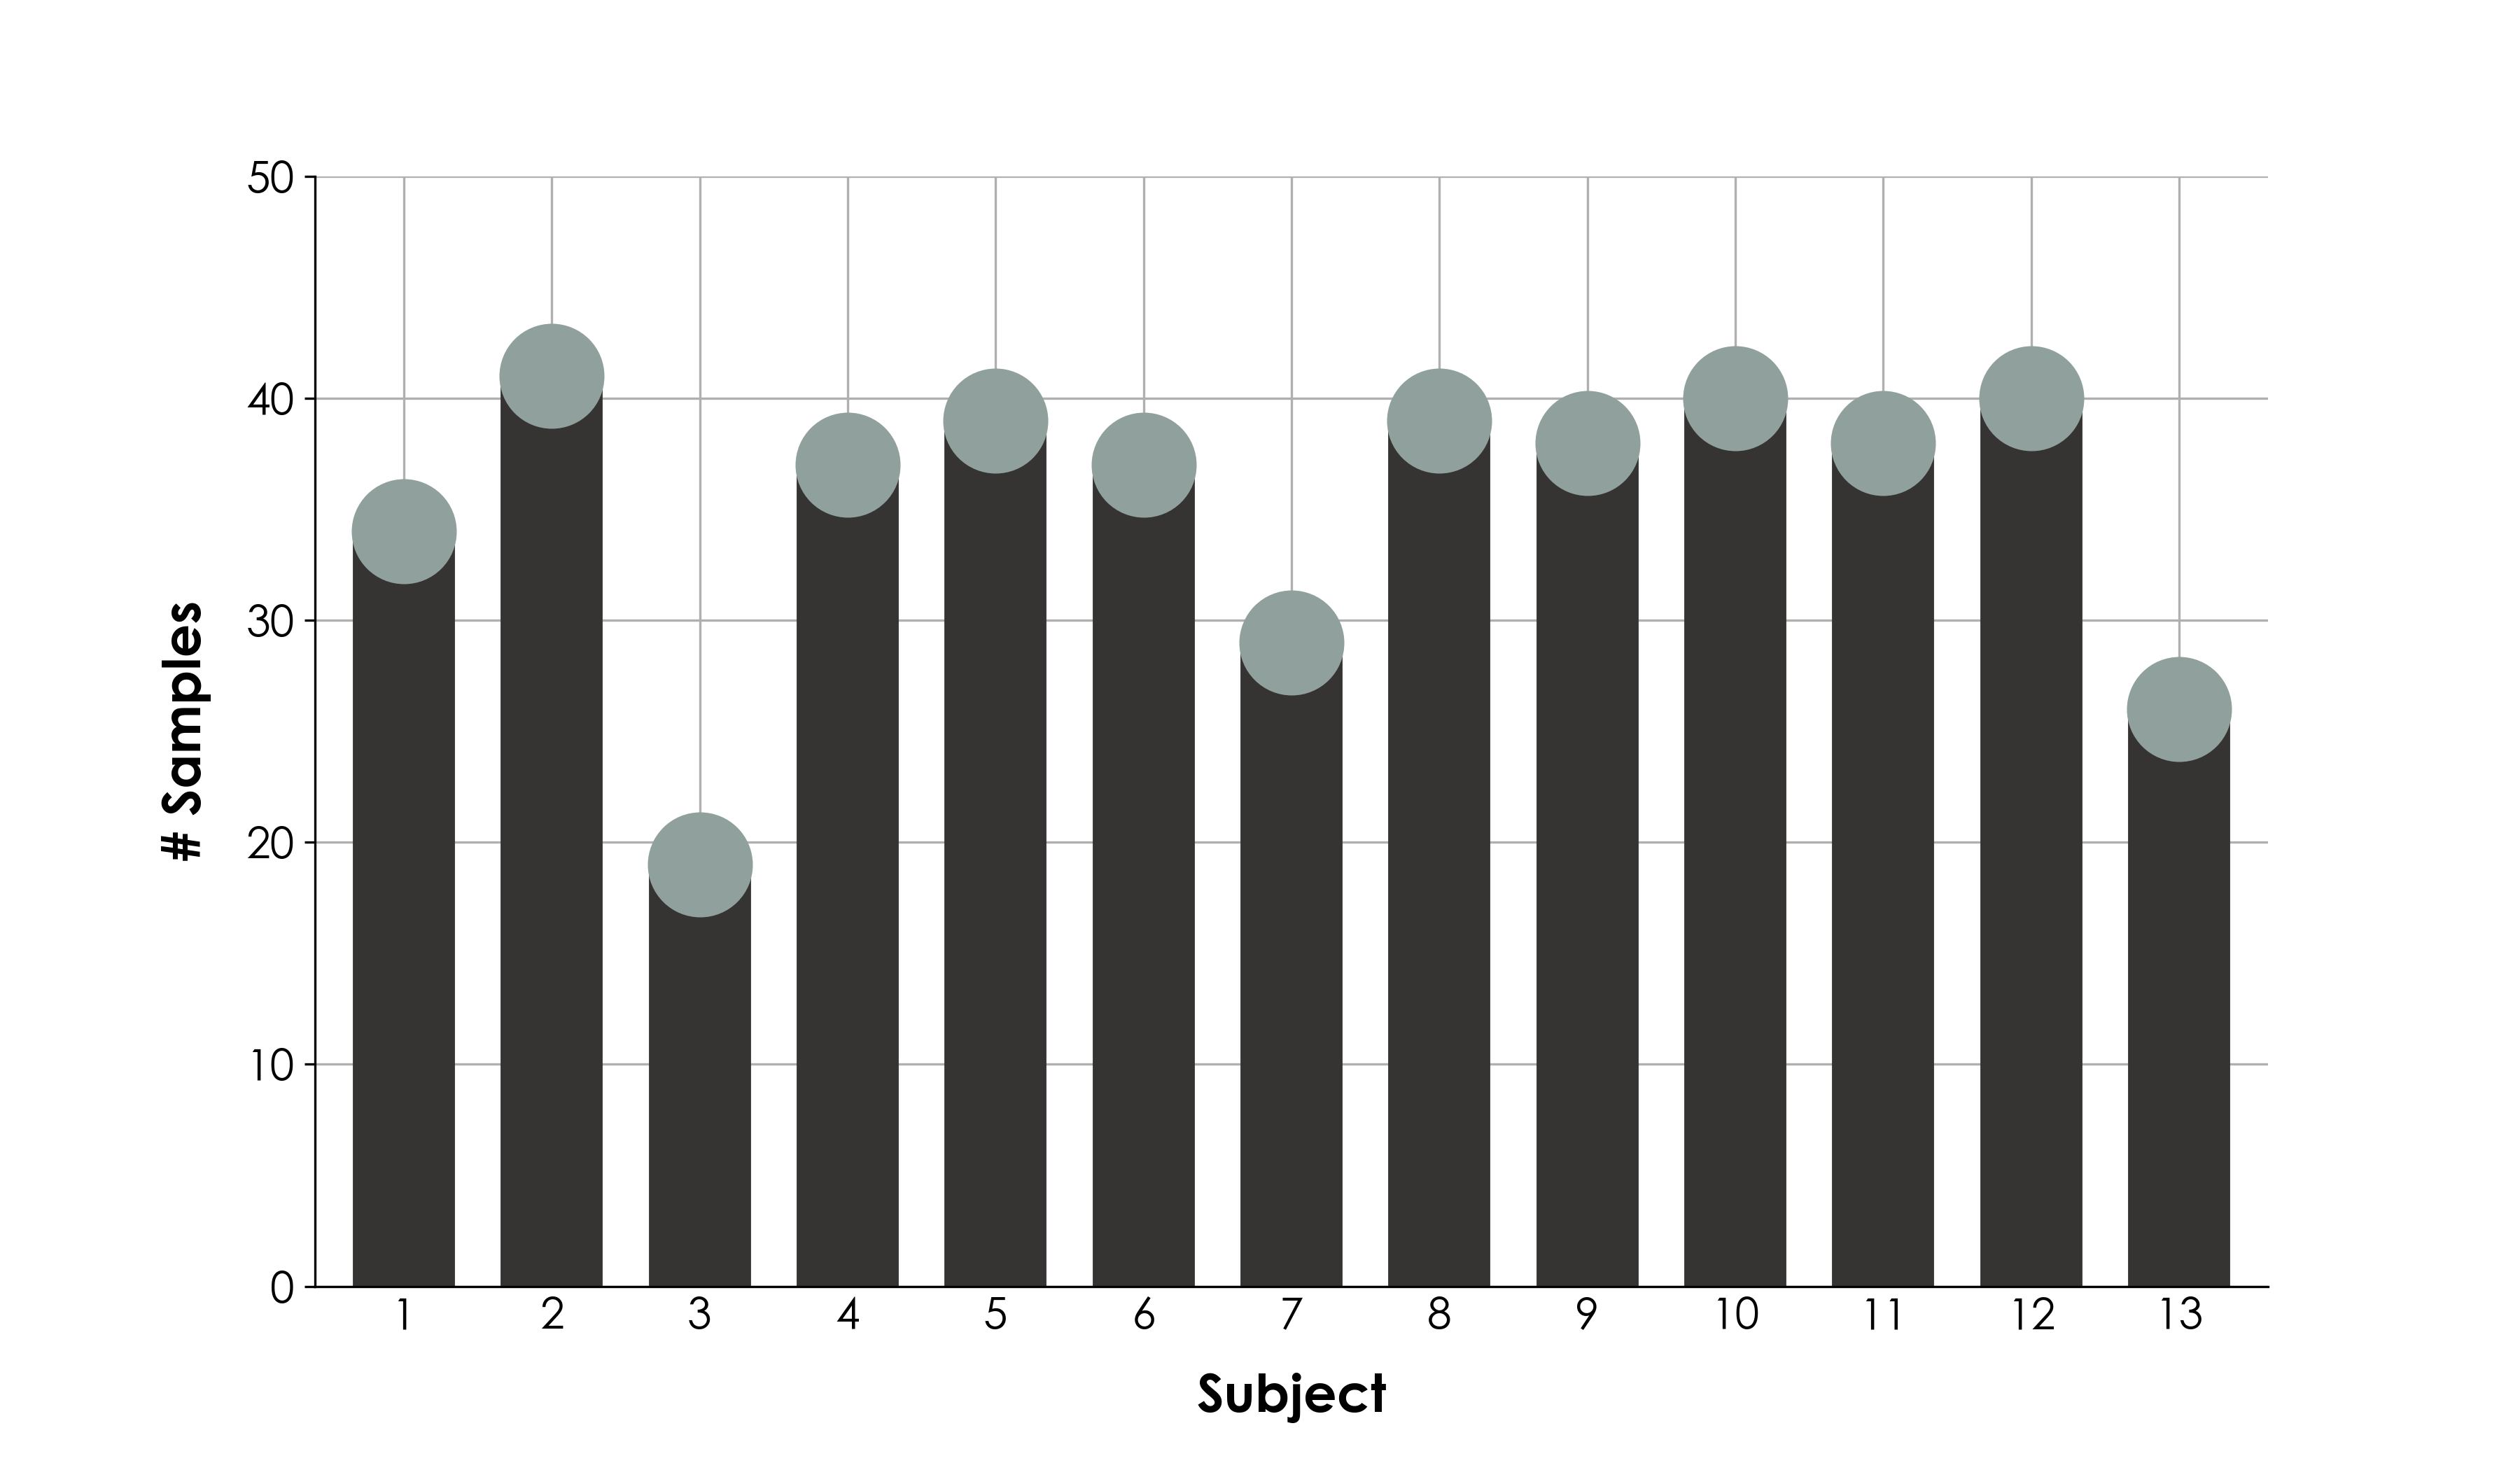
\includegraphics[width=1.0\textwidth]{./figure/chap 4/subjectwise_data_counts}
\caption{Number of samples by subject}
\label{Fig 4.10}
\end{figure}

\subsection{Dataset Summary}
Different aspects of the dataset is summarized in \ref{Table 4.3}.

\begin{table}[H]
\caption{Dataset summary}
\vspace{2mm}
\centering
\begin{tabular}{|l|c|} 
\hline
\multicolumn{1}{|c|}{\textbf{Specification}} & \multicolumn{1}{c|}{\textbf{Value}}                                                      \\ 
\hline
Device used             & ESP32-WROOM-32E             \\
Signals used            & CSI, RSSI                   \\
Activities              & 5                           \\
Subjects                & 13                          \\
Subject age range       & 18-25                       \\
Total samples           & 966                         \\
Selected samples        & 898                         \\
Sampling rate           & 100 Hz                      \\
Each sample time window & 4 seconds                   \\
Mean packet count       & 287                         \\
Room temperature        & 25 $^{\circ}$ C             \\
\hline
\end{tabular}
\label{Table 4.3}
\end{table}


\section{Data Preprocessing Pipeline}
The data we collected includes the raw signal information and packets. In this section, we propose a robust and complex preprocessing pipeline to preprocess the raw data and make the raw data used for the system. At first, we need to extract the CSI data from the raw signal and isolate the phase and amplitude information from it. As CSI data is inherently sensitive to different environmental parameters, some cleaning process needs to be applied such as calibration, denoising, and dimensionality reduction. There are various denoising algorithms to choose from. We compare their performances and choose the best one. After preconditioning the signals, we feed the data to the feature extraction module that extracts different features from the cleaned data. Not all the features are important for the outcome. So, we have to use different mathematical models to find the most relevant features. A normalization technique is employed before handing the data over to a competent machine learning model. Lastly, we tune different hyperparameters of the model to increase the performance of the model on the dataset. 

\begin{figure}[H]
\centering
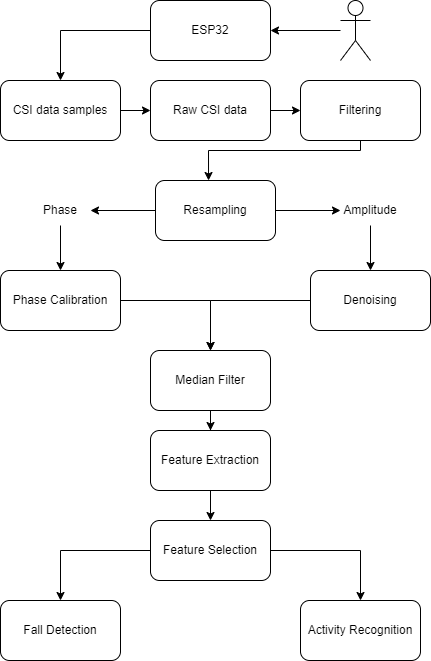
\includegraphics[width=0.7\textwidth]{./figure/chap 4/csiProject.drawio.png}
\caption{Complete Pipeline of The System}
\label{Fig 4.11}
\end{figure}

\subsection{CSI Data Extraction}
CSI essentially enables us to comprehend what transpires on the channel between the transmitter and receiver. CSI is calculated by examining how the preamble with known content is changed during transmission. Thus, we have a collection of complex numbers in the form $a_{n} \exp j \theta_{n}$, where $a_{n}$ is the amplitude and $ \theta_{n}$ is the phase. We need to extract this amplitude and phase from the raw CSI data. A raw CSI packet comprises the real and imaginary part of the channel state and is transmitted separately for each subcarrier. But not all subcarriers carry useful information. Different subcarriers respond differently to human activity; for example, certain subcarriers are quite sensitive to motion and exhibit obvious fluctuations. It is preferable to use only the CSI information from these sensitive subcarriers. The computing complexity of the system is also increased by using all of the data from all of the subcarriers. So, we removed some of the irrelevant subcarriers by examining the acquired CSI sequence, and skillfully isolate the signal segments mostly corresponding to human activity. Then we transformed the real and imaginary parts of the selected subcarriers into polar form to get the required amplitude and phase information.

\subsection{Time Series Representation}
The extracted CSI data ideally should be a time series having a constant time difference between two samples. But in practice, the sampling rate was not constant and there was a considerable amount of packet loss which led to non-uniform data. To apply different time and frequency domain analysis, this data need to convert to a time series representation. That's why we resampled the data at a constant 100 Hz sampling rate. This process involves resulting in some missing values which are linearly interpolated to generate an equivalent waveform.

\begin{figure}[H]
\centering
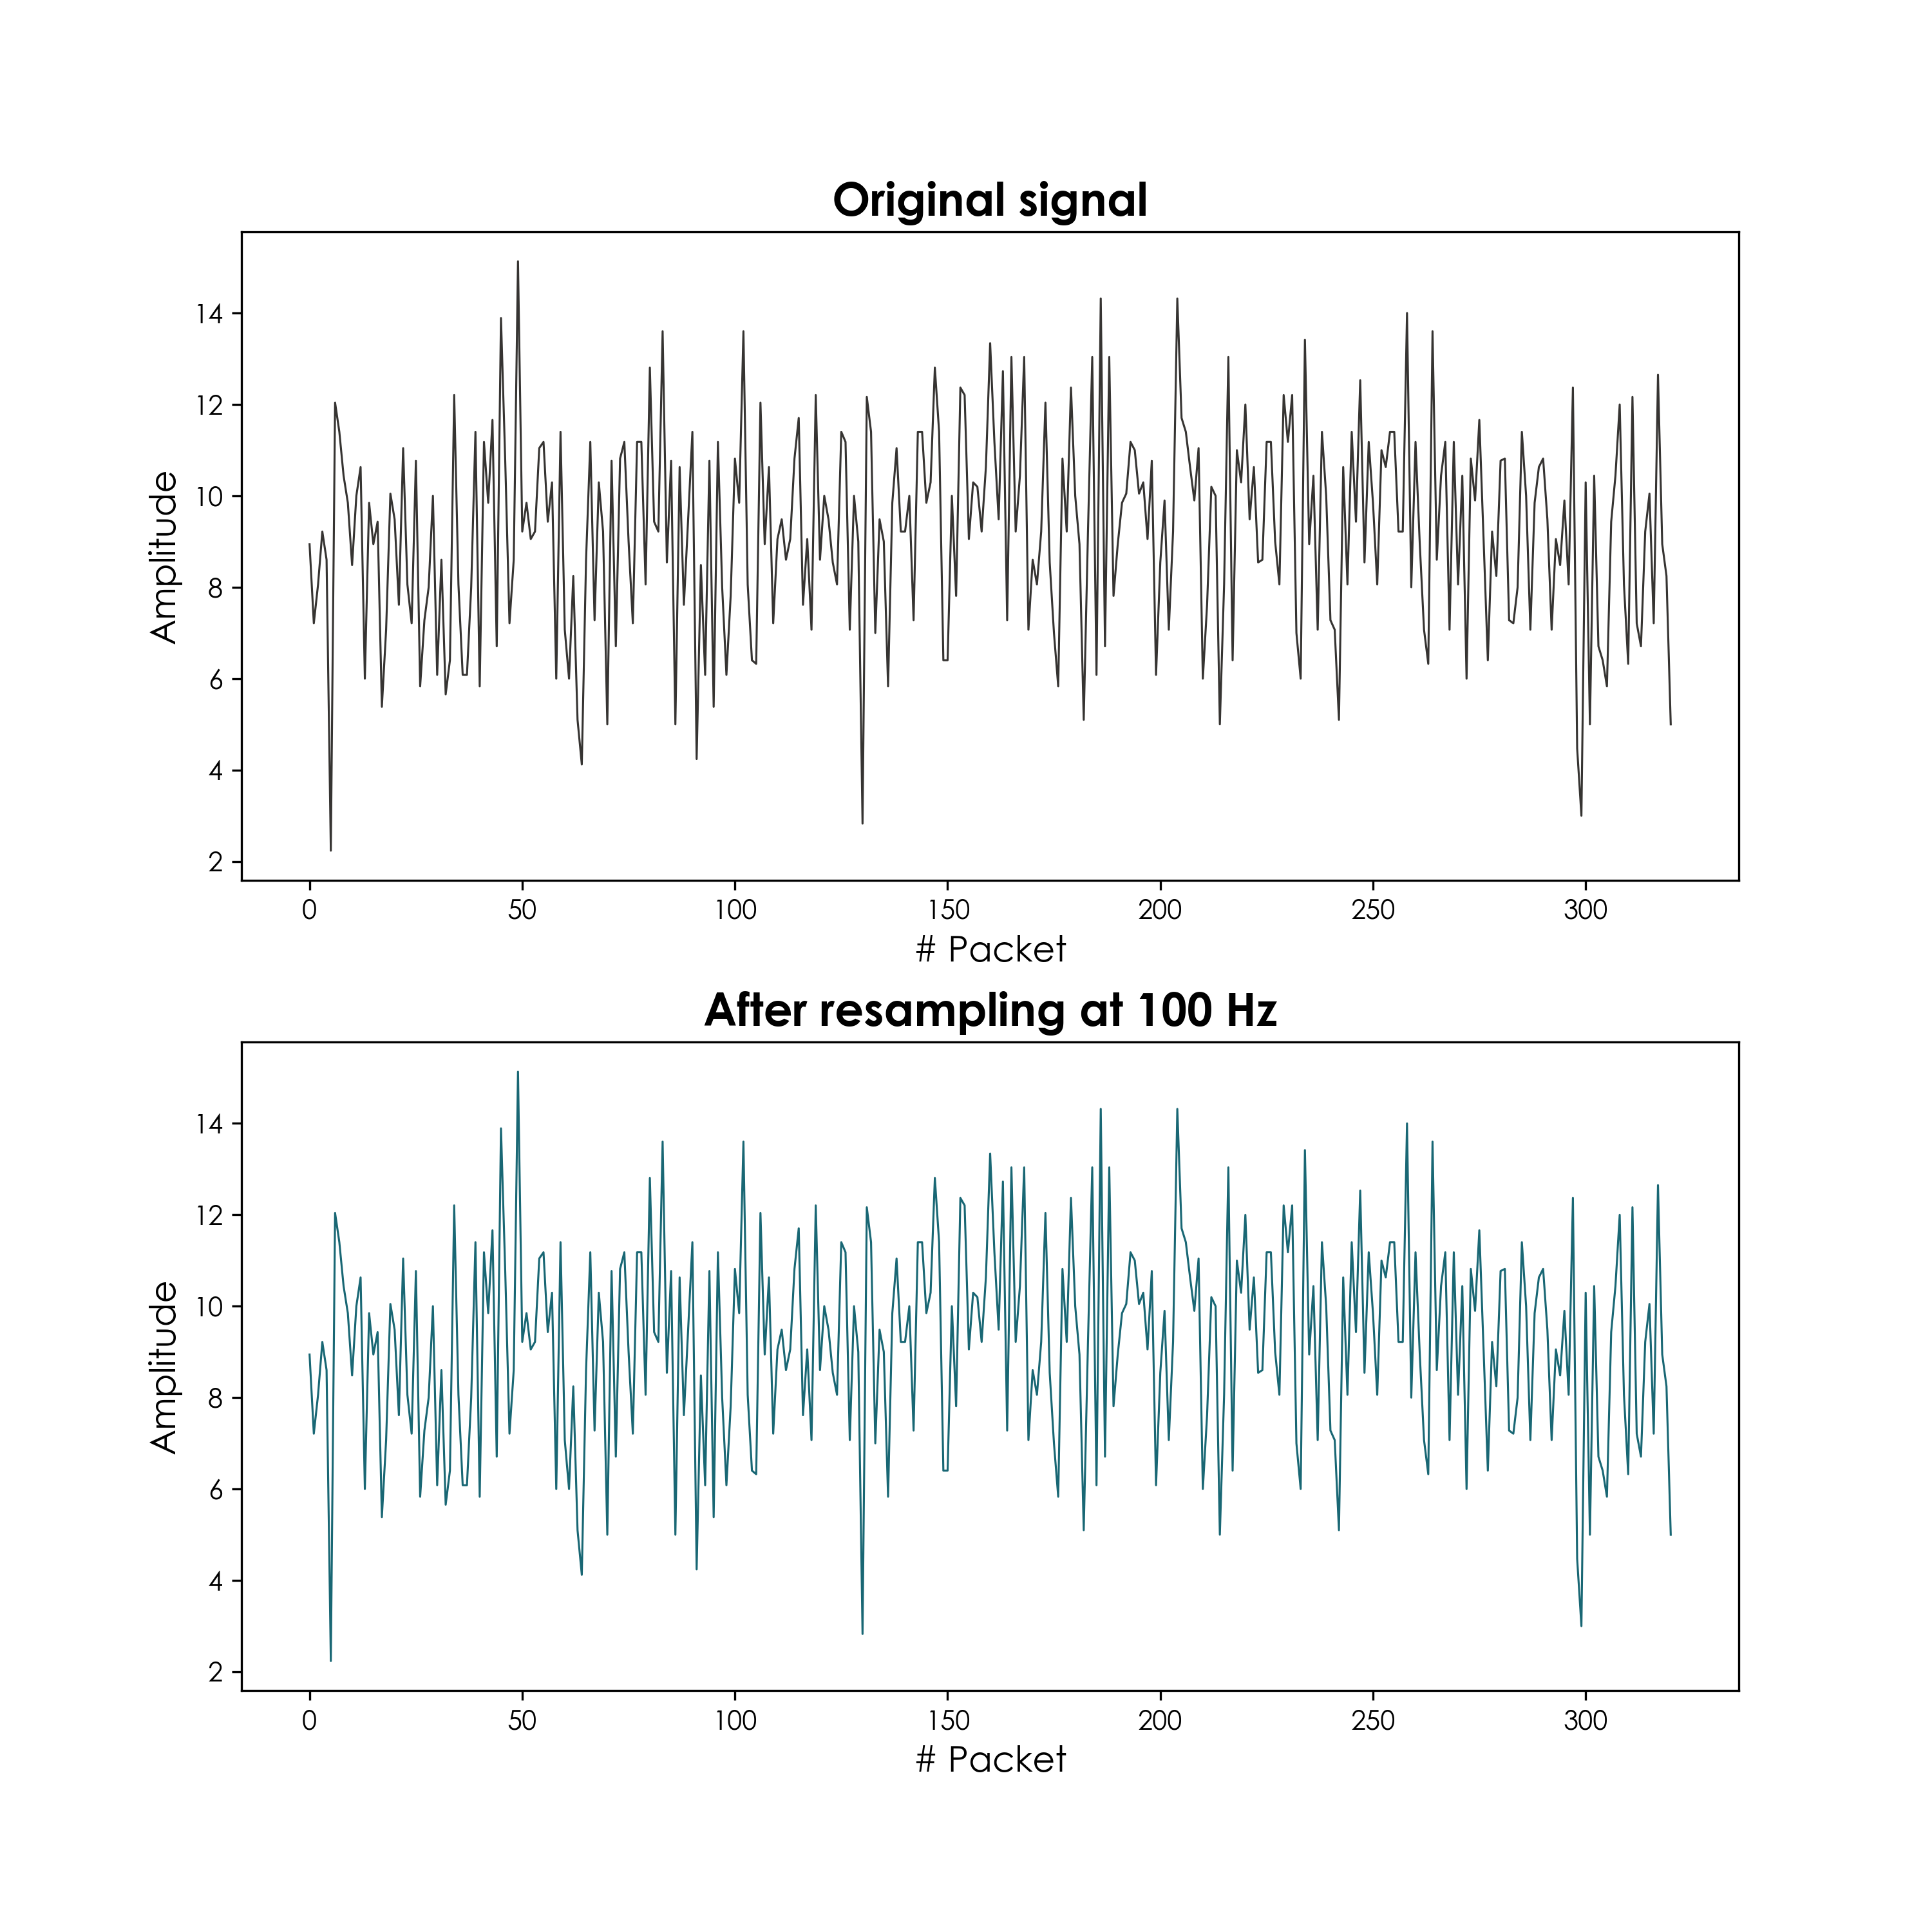
\includegraphics[width=1.0\textwidth, trim={0 1cm 0 0} , clip]{./figure/chap 4/resampling_plot.png}
\caption{Resampling for time series representation}
\label{Fig 4.12}
\end{figure}


\subsection{Phase Signal Analysis}
The isolated phase information of $i^{th}$ subcarrier can be expressed by the following equation:
\begin{equation}
    \hat{\phi _i} = \phi _i - 2\pi \frac{s_i}{N}\tau + \beta + Z
\end{equation}
Here, $\phi_i$ is the actual phase which is deteriorating by the time offset at receiver $\tau$, unknown time offset $\beta$, and measurement error $Z$. $s_i$ is the subcarrier index and $N$ signifies the Fast Fourier Transform (FFT) size which is 64 for IEEE 802.11n. Due to this distortion, the phase must be calibrated the restore the actual phase as much as possible. As shown by \cite{10.1145/2307636.2307654}, the time offsets, $\tau$, and $\beta$ can be removed by considering the phase across the frequency band given by the equation:
\begin{equation}
    \hat{\phi _i} =  \hat{\phi _i} - as_i - b =  \hat{\phi _i} - \frac{\phi _n - \phi _1}{s_n - s_1} s_i - \frac{1}{n} \sum_{j=1}^{n} \phi _j
\end{equation}
Here, $a$ and $b$ are intermediate variables. 
But in this process, the true phase is folded due to
the recurrence characteristic of the phase. This problem can be solved by compensating multiple $2\pi$’s by judging whether the measured phase change between the adjacent subcarriers is greater than the given thresholds \cite{7460092}.

\subsection{Denoising Amplitude Signal}
The amplitude of the CSI data is very sensitive to internal and external noises. Possible noise sources are scattering, reflection, delay, fading, and power line losses. The signal can be denoised by using various techniques including different filters or transformations.

\begin{figure}[H]
\centering
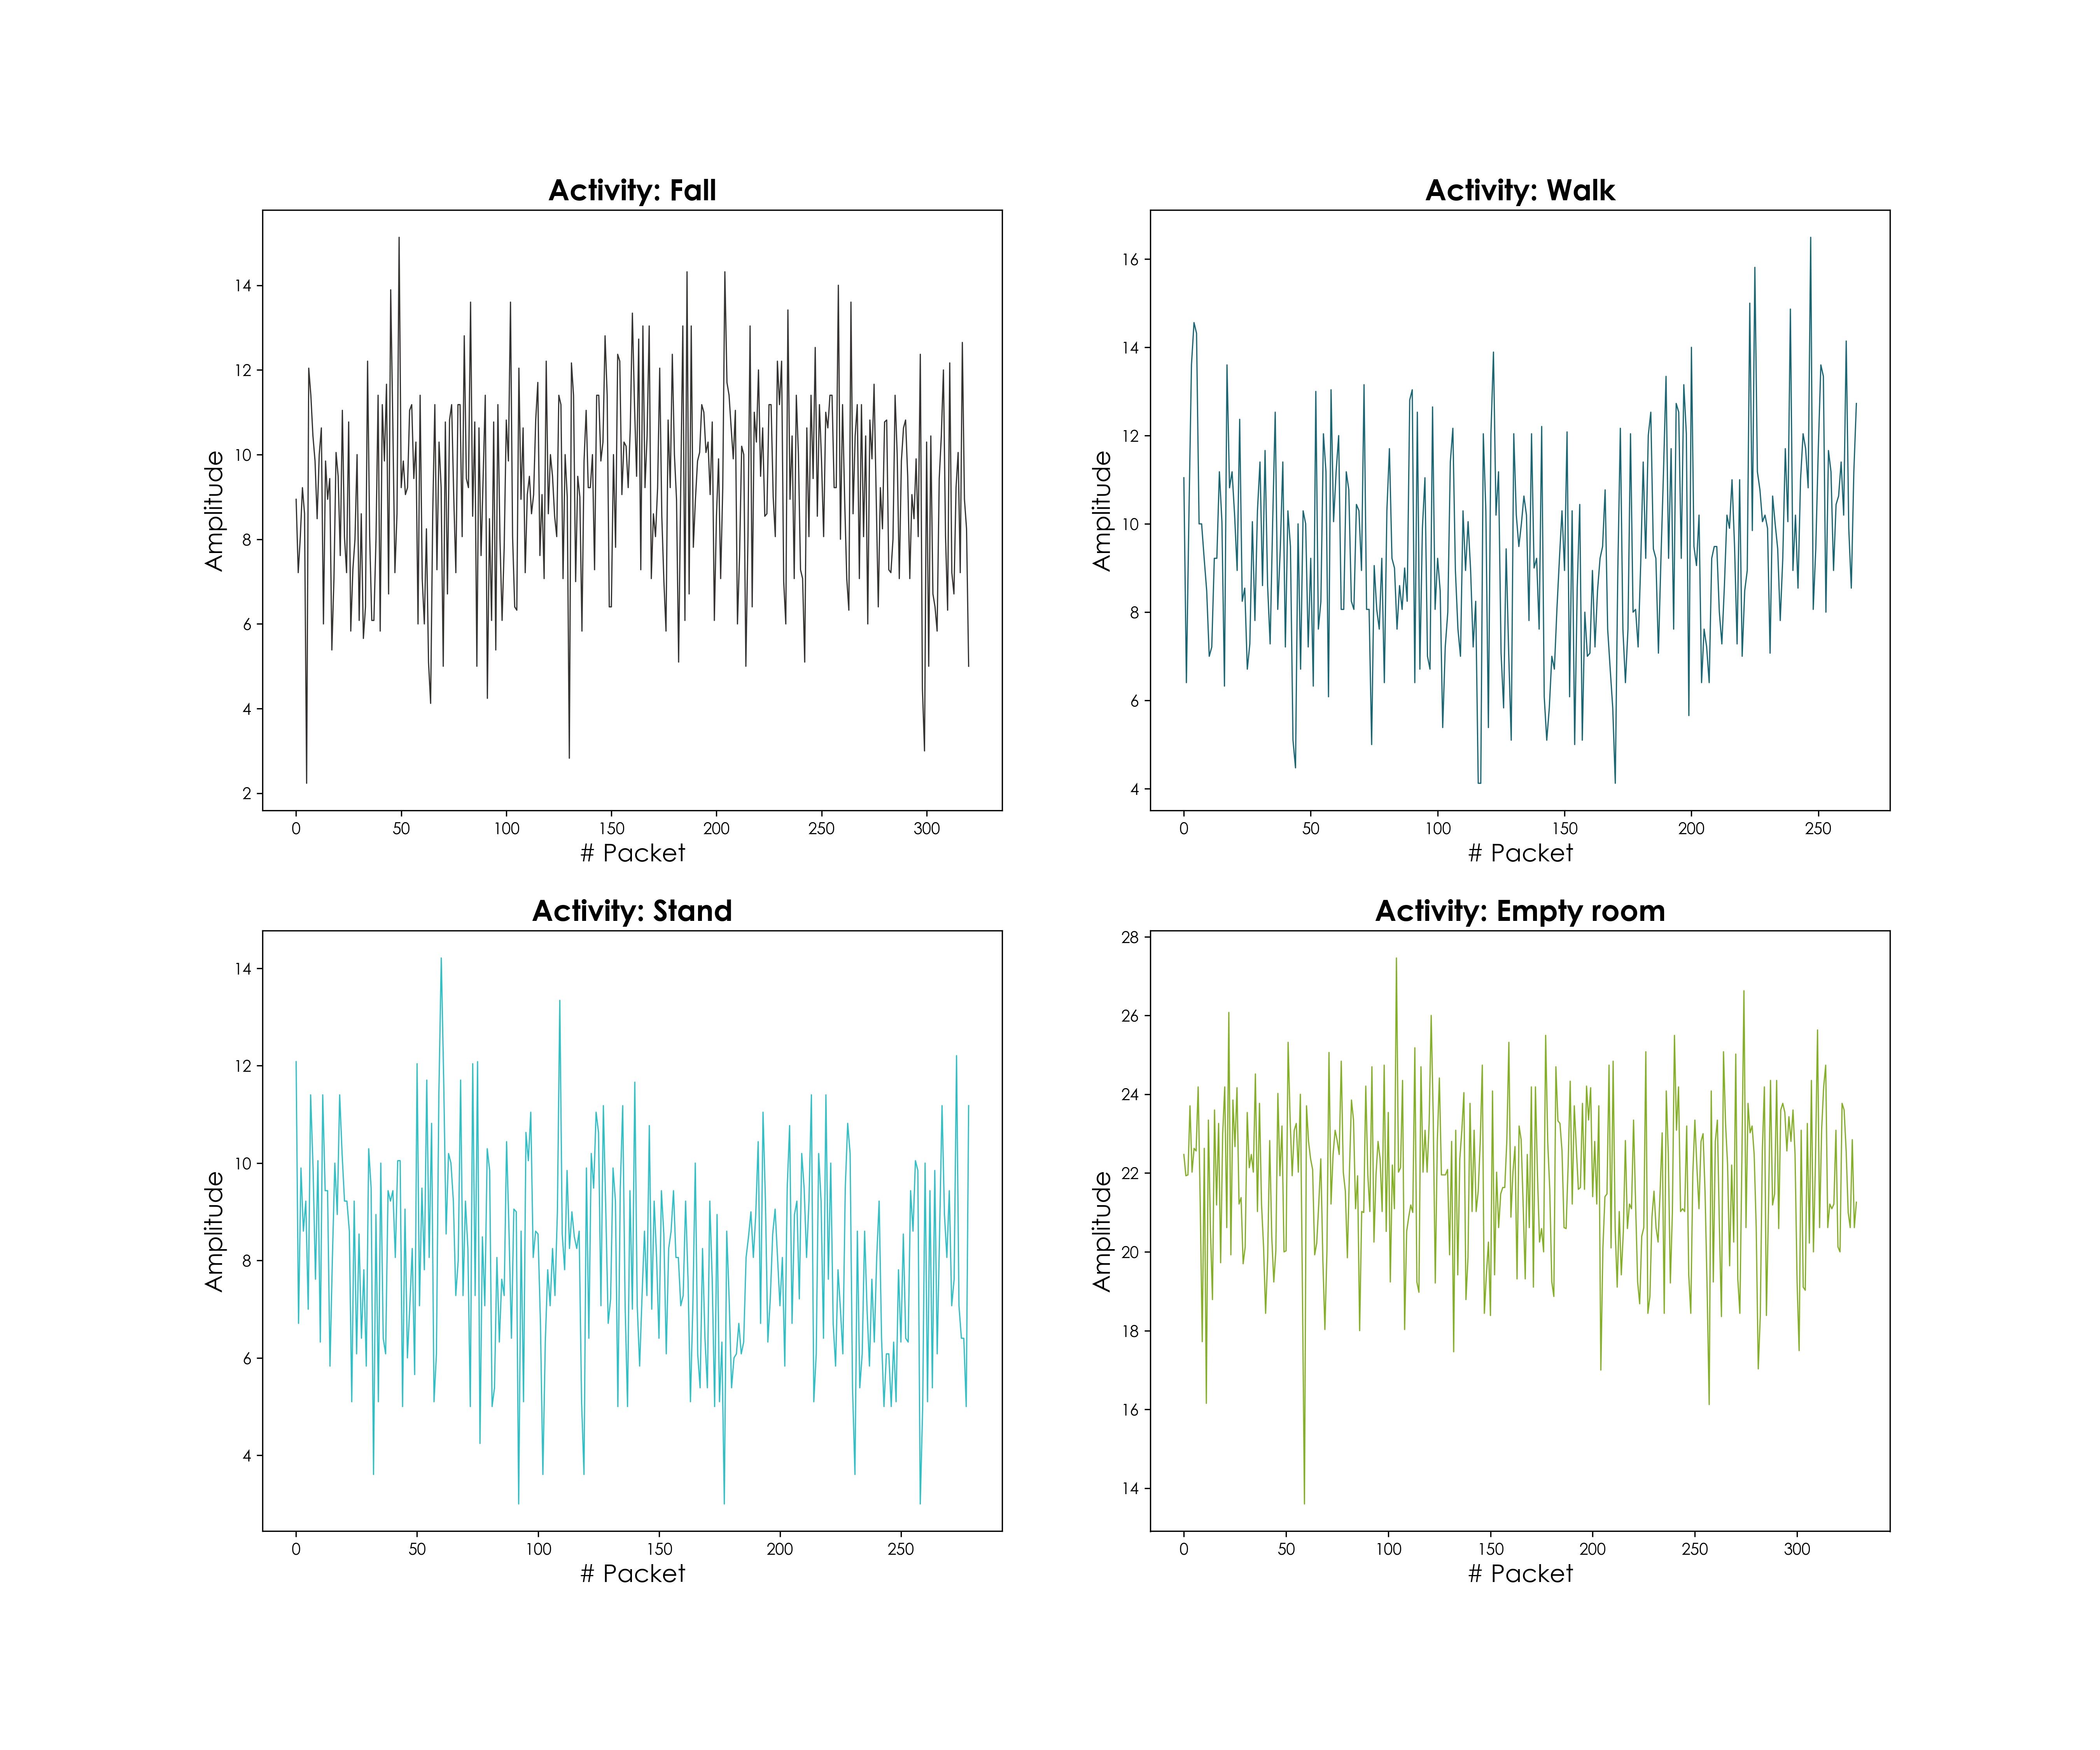
\includegraphics[width=1.0\textwidth, trim={0 3cm 0 2cm},clip]{./figure/chap 4/magnitude_plot_raw.png}
\caption{Raw CSI amplitude signal for different activities}
\label{Fig 4.13}
\end{figure}

\subsubsection{Low Pass Filter (LPF)}
A low-pass filter is a filter that attenuates the higher frequency portion of a signal than a chosen cutoff frequency. The filter's precise frequency response is determined by the filter's design. There are many types of low pass filters, but in this project, we will focus on a specific type named \emph{Butterworth filter} \cite{butterworth1930theory}. Butterworth filter is a signal processing filter made to have a frequency response that is as flat as possible in the passband.  Butterworth filter has a slower roll-off and thus will require a higher order to implement a particular stopband specification, but it has a more linear phase response in the passband than most others. Low pass butterworth filters are greatly used for noise removal from various signals. Generally, a noisy wave contains two different portions: high-frequency noise and low-frequency true signal. This also fits for CSI amplitude signal. Thus the high-frequency noise mixed in the signal can be removed by using a Butterworth low pass filter. But a problem with this method arises when the signal and noise frequency are not separated by a large margin. As butterworth filter has a slower roll-off, it tends to attenuate some of the original signals too. 

\subsubsection{Fast Fourier Transform (FFT)}
A fast Fourier transform (FFT) algorithm calculates a sequence's discrete Fourier transform (DFT) or its inverse (IDFT). Through the process of Fourier analysis, a signal is transformed from its original domain, which is frequently time or space, to a representation in the frequency domain, and vice versa. The DFT is produced by breaking down a series of numbers into components of various frequencies. [1] Although computing it straight from the specification is generally too time-consuming to be helpful, this technique has many applications. Such changes are quickly computed by an FFT by factorizing the DFT matrix into a product of sparse (mostly zero) elements.\cite{fft} This successfully reduces the complexity from    $O(N^2)$ to  $O(Nlog(N))$ where N is the number of samples.

\subsubsection{Short-Time Fourier Transform (STFP)}
A Fourier-related transform known as the Short-time Fourier transform (STFT) is used to ascertain the sinusoidal frequency and phase content of local parts of a signal as they change over time. To compute STFTs, it is necessary to split a longer temporal signal into equal-length shorter segments. Each shorter segment is then subjected to a separate Fourier transform computation. This makes each shorter segment's Fourier spectrum visible. The shifting spectra are then typically plotted as a function of time using a technique called a spectrogram or waterfall plot, which is frequently applied in Software Defined Radio (SDR)-based spectrum displays. On desktop PCs, Fast Fourier Transforms (FFTs) with $2^{24}$ points are frequently used for full bandwidth displays that span the whole SDR range.\cite{stft}

\subsubsection{Wavelet Transform (WT)}
In Fourier transform (FT), we represent a function using a series of sine and cosine waves, which is an excellent approach to understanding the frequencies present in the signal. However, it has a significant drawback. FT only contains the frequency information, but the spatial or temporal information is completely lost. It will not be possible to tell where the frequency is low or high in the space or time domain, or where frequency shifts are taking place. To overcome this problem, we do Wavelet Transform (WT). In WT, we represent a function using a certain orthonormal series produced by a wavelet. A wavelet is a waveform of effectively limited duration that has an average value of zero and nonzero norm. If a function $\phi$ can provide a Hilbert basis or a full orthonormal system, for the Hilbert space of square-integrable functions, then $\phi$ is referred to as an orthonormal wavelet. The fundamental principle of wavelet transform is that they should only be able to modify the length of time, not shape. This is impacted by selecting appropriate base functions that support this. Changes to the time extension should match up with the analysis frequency of the basis function. 

\subsubsection{Discrete Wavelet Transform (DWT)}
A discrete wavelet transform (DWT) \cite{shensa1992discrete} decomposes an input signal into several sets, each set consisting of a time series of coefficients that describe the signal's temporal evolution in the associated frequency band. In this process, the wavelets are sampled in discrete steps. A key advantage it has over Fourier transforms is temporal resolution: it can show both frequency and location information (location in time). The DWT refers not just to a single transform, but rather to a set of transforms, each with a different set of wavelet basis functions. Two of the most common are the Haar wavelets and the Daubechies set of wavelets. Unlike the Continuous Wavelet Transform (CWT), it uses a finite set of wavelets, i.e., defined at a particular set of scales and locations. But the main idea remains the same; we multiply the signal with a particular wavelet with a particular scaling and then shift it over the whole signal to integrate. In DWT, we repeat the procedure after changing the scale. In these situations, scaling adjustments are made discretely.
The DWT can be defined by the following equation:
\begin{equation}
    T_{m,n} = \int_{-\infty}^{\infty} x(t) \psi _{m,n} (t) dt 
\end{equation}

where $\psi$ is the wavelet function. The components of the signal can be assembled back into the original signal without loss of information using a reconstruction algorithm known as the Inverse Discrete Wavelet Transform (IDWT). In IDWT, the DWT coefficients are first upsampled by inserting zeros between each coefficient, essentially doubling the length of each (the approximation and the detail coefficients are handled separately). The reconstruction scaling filter for approximation coefficients and the reconstruction wavelet filter for detail coefficients are then convolved with these. To get the original signal, these results are then put together. 

\subsubsection{Comparison of DWT and LPF}
For our dataset, we employed two different types of denoising methods. One is a $4^{th}$ order Butterworth low pass filter with a cut-off frequency of 10 Hz. The other is a second-level Discrete Wavelet Transform using symlet10 wavelet. 

\begin{figure}[H]
\centering
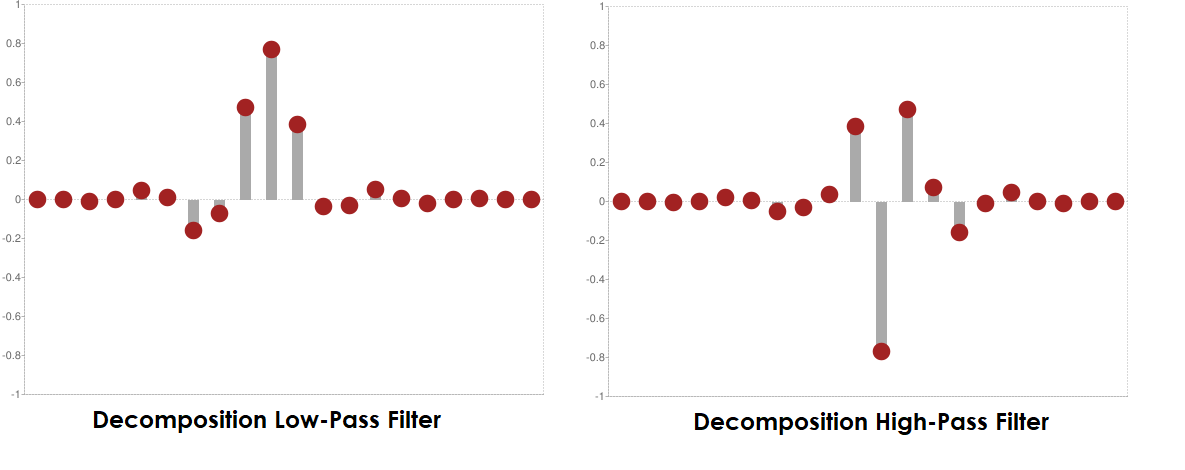
\includegraphics[width=1.0\textwidth]{./figure/chap 4/sym10.png}
\caption{Symlet10 wavelet}
\label{Fig 4.14}
\end{figure}

We used both denoisers and compared how they work on different CSI amplitude waves. By careful comparison, we found the DWT denoising method performed better than low pass filter. So, we chose DWT denoising for this system.

\begin{figure}[H]
\centering
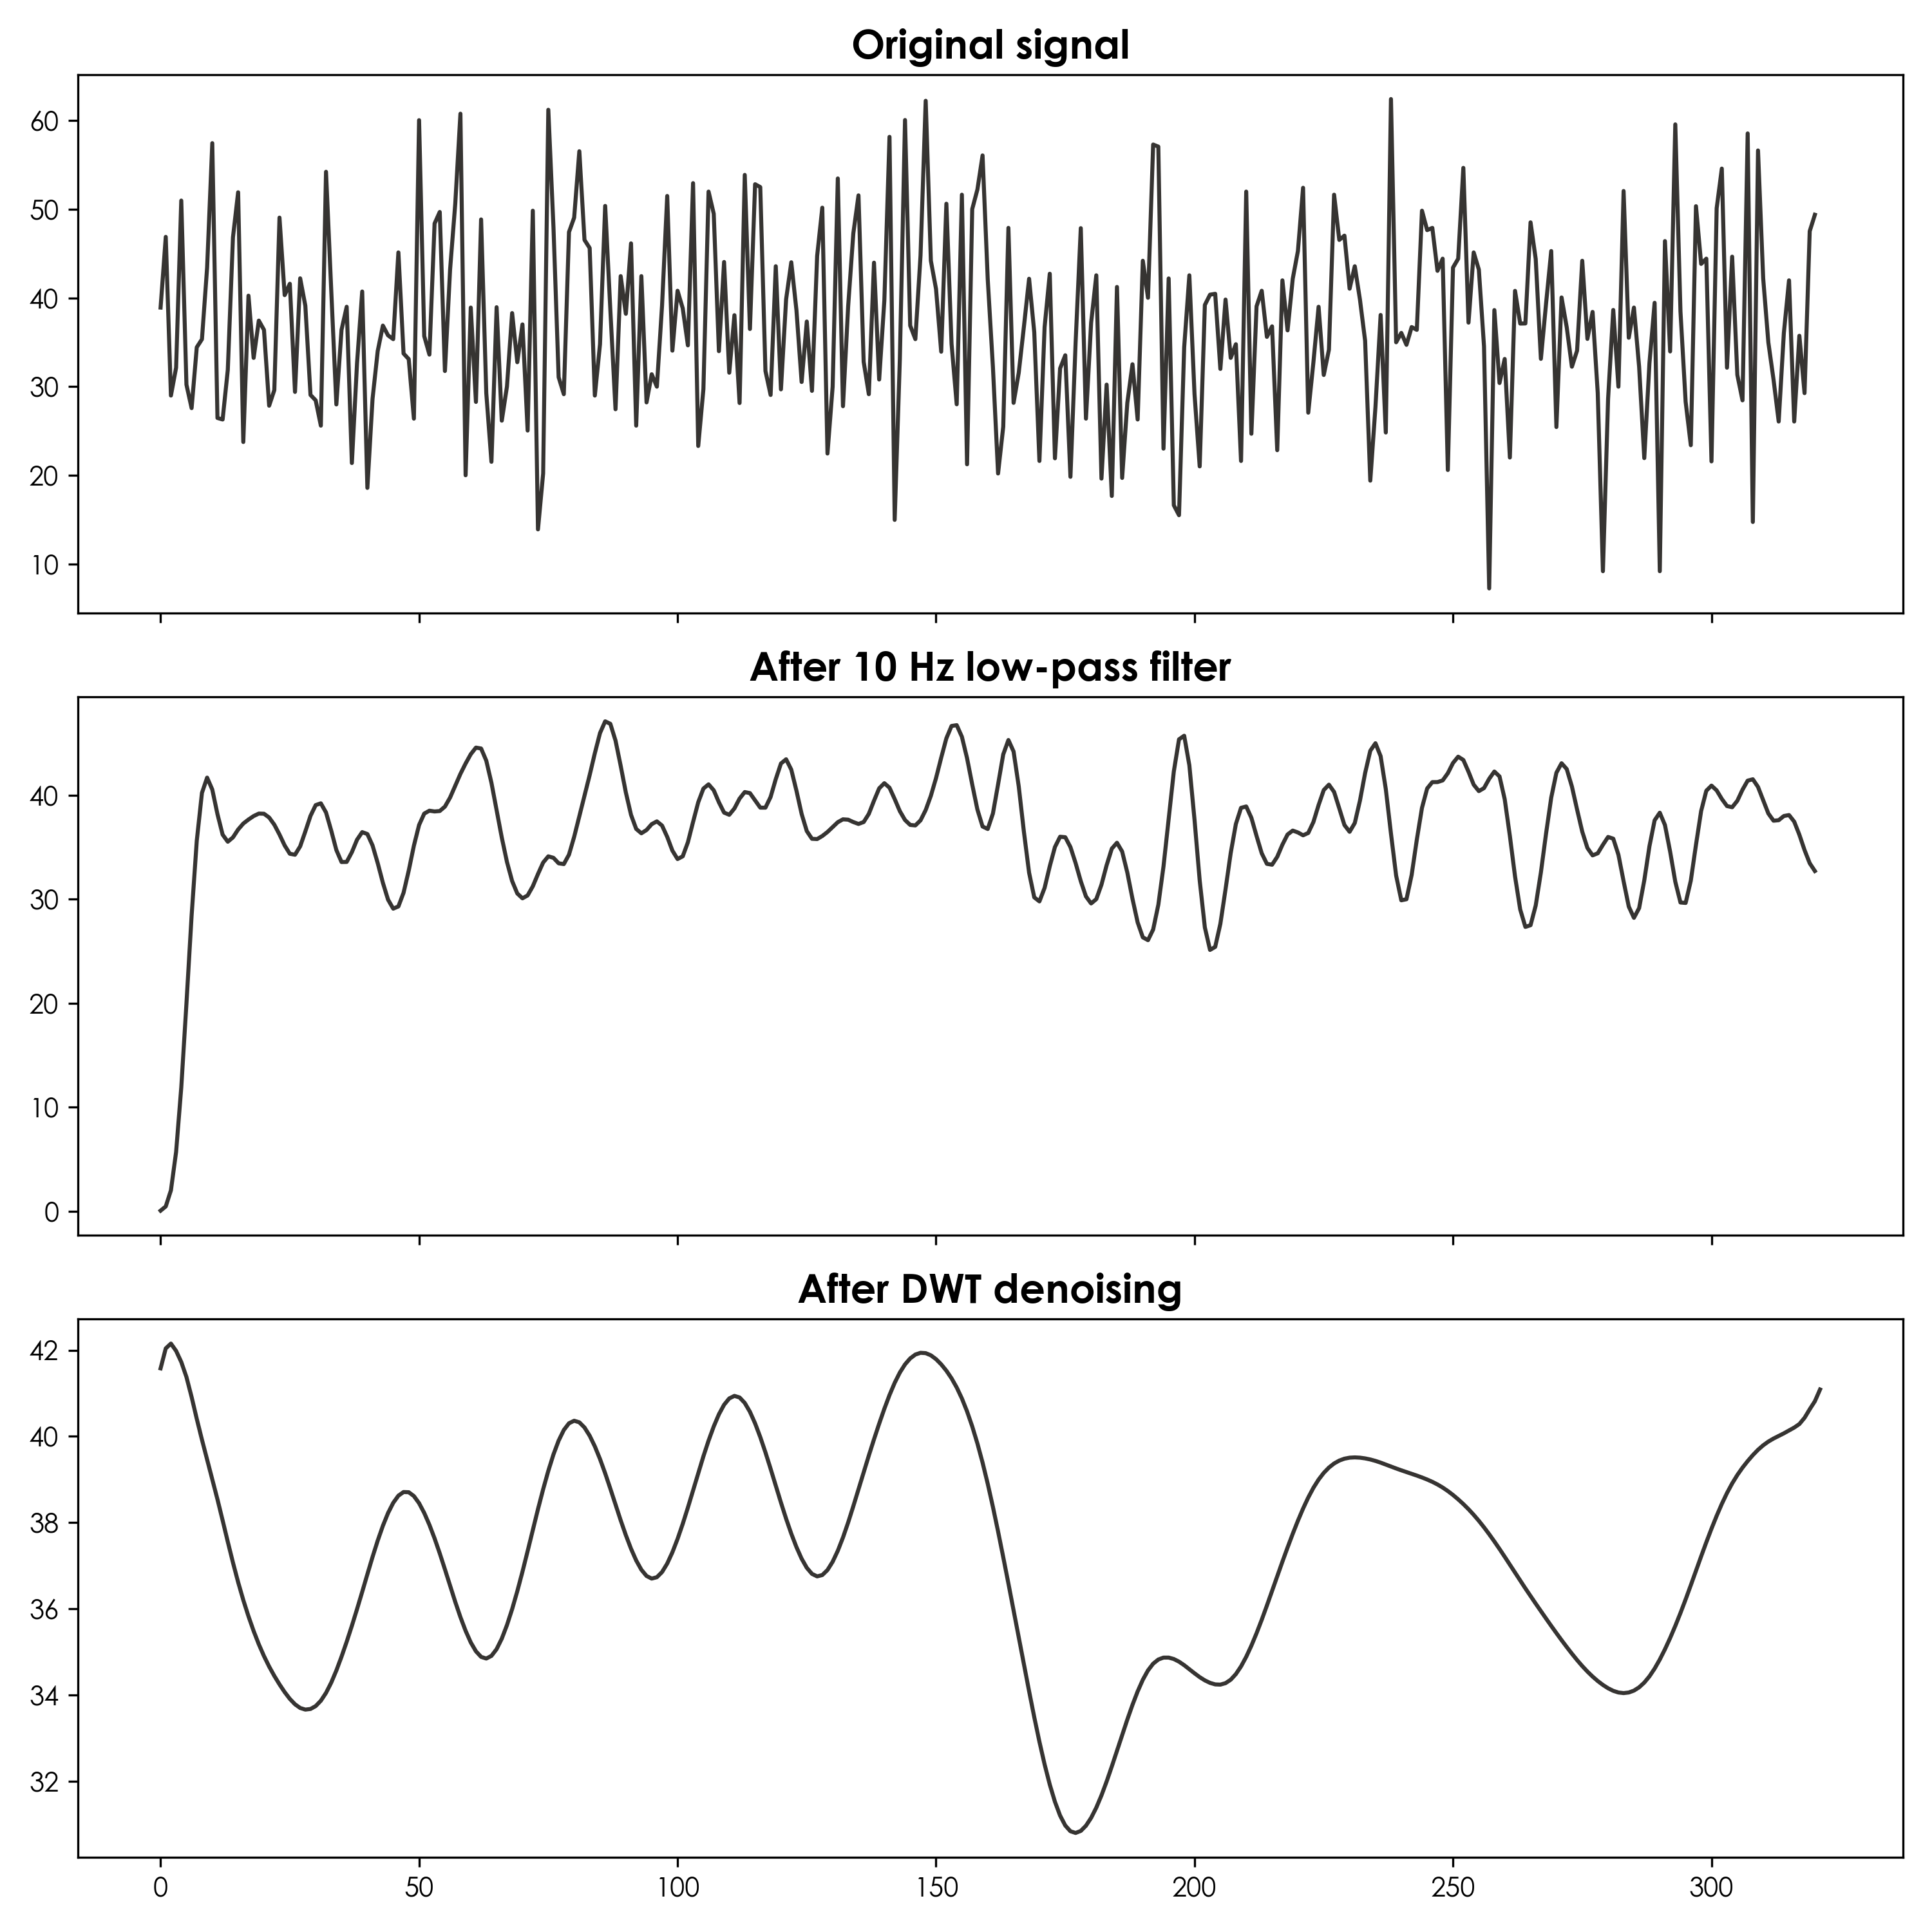
\includegraphics[width=1.0\textwidth]{./figure/chap 4/lpf_vsdwt.png}
\caption{Comparison between low pass filter and DWT}
\label{Fig 4.15}
\end{figure}

\section{Feature Selection}
After conditioning and denoising the signals, we extracted some statistical features including min, max, median, and standard deviation from the phase and amplitude CSI and RSSI signals. But the initial feature size was 716 which is very large considering the sample size which is only 898. So, we needed to prune the feature set to remove non-correlated features. There are different ways to measure the correlation or importance of the features with the output variable.

\subsection{Chi-Square Test \cite{chisquare}} 
One technique to demonstrate a connection between two categorical variables is via a chi-square statistic. The chi-squared statistic is a single figure that indicates the degree to which the counts you saw deviate from the counts you would anticipate if there were no association at all in the population. 

\begin{equation}
    \chi_c^2 = \sum \frac{(O_i - E_i)^2}{E_i}
\end{equation}

\subsection{Pearson's Correlation Coefficient (PCC) \cite{pcc2020}}
Pearson’s correlation coefficient is the test statistics that assess the statistical association, or relationship, between two continuous variables. Because it is based on the method of covariance, it is regarded as the best method for determining the relationship between variables of interest. It provides details on the size of the association or correlation as well as the relationship direction. One problem with PCC is that it is not able to tell the difference between dependent variables and independent variables.

\subsection{Decision Tree (DT) based feature selection \cite{dtfeatureselection}}
Decision tree building algorithm selects the splits locally, i.e. concerning the splits selected in earlier stages, so that the features occurring in the decision tree, are complementary. Thus, Decision Tree based models provide feature importance metrics that can be utilized to select the most important features. 

We used a combination of PCC and decision tree-based selection methods to select the most important 243 features for our proposed method.


\section{Training Description}
Every supervised machine learning system has three phases: 
\begin{enumerate}
    \item Training phase: We train the data for the known labels.
    \item Testing phase: We evaluate the performance of the trained model keeping the labels away from the model.
    \item Application phase: We apply our model for real-life unknown data.
\end{enumerate}

Our proposed preprocessing pipeline is independent of the training phase. So, it gives us the advantage to use any machine learning model for our preprocessed data even for different learning tasks. In this project, we have two different learning objectives. One is \emph{fall detection} and the other one is a generalized \emph{human activity recognition}. 
\subsection{Fall Detection}
For fall detection, we classified the \emph{walk} and \emph{stand} activities as non-fall activity, kept the \emph{fall} activity as is and did not use the \emph{empty room} and \emph{presence} activities. Then, we trained binary classification algorithms on this data.
\subsection{Human Activity Recognition}
In this objective, we utilized the whole dataset with all the activities, i.e., \emph{fall}, \emph{stand}, \emph{walk}, \emph{empty room} and \emph{presence}. So, we have five labels in this task and used this data in different multi-class classification algorithms.

In both cases, we compared the behavior and performance of these algorithms and tuned them to get the best performance on the test set. The performance statistics of these models are depicted in the next chapter.

